\pdfoutput=1
% Options for packages loaded elsewhere
\PassOptionsToPackage{unicode}{hyperref}
\PassOptionsToPackage{hyphens}{url}
\PassOptionsToPackage{dvipsnames,svgnames,x11names}{xcolor}
%
\documentclass[
  10pt,
]{article}
\usepackage{amsmath,amssymb}
\usepackage{iftex}
\ifPDFTeX
  % T1 fontenc omitted: OT1 Computer Modern (Type 1)
  \usepackage[utf8]{inputenc}
  \usepackage{textcomp} % provide euro and other symbols
\else % if luatex or xetex
  \usepackage{unicode-math} % this also loads fontspec
  \defaultfontfeatures{Scale=MatchLowercase}
  \defaultfontfeatures[\rmfamily]{Ligatures=TeX,Scale=1}
\fi
% lmodern omitted
\ifPDFTeX\else
  % xetex/luatex font selection
\fi
% Use upquote if available, for straight quotes in verbatim environments
\IfFileExists{upquote.sty}{\usepackage{upquote}}{}
\IfFileExists{microtype.sty}{% use microtype if available
  % microtype omitted
  % % disable protrusion for tt fonts
}{}
\makeatletter
\@ifundefined{KOMAClassName}{% if non-KOMA class
  \IfFileExists{parskip.sty}{%
    \usepackage{parskip}
  }{% else
    \setlength{\parindent}{0pt}
    \setlength{\parskip}{6pt plus 2pt minus 1pt}}
}{% if KOMA class
  \KOMAoptions{parskip=half}}
\makeatother
\usepackage{xcolor}
\usepackage[margin=2.2cm]{geometry}
\usepackage{longtable,booktabs,array}
\usepackage{calc} % for calculating minipage widths
% Correct order of tables after \paragraph or \subparagraph
\usepackage{etoolbox}
\makeatletter
\patchcmd\longtable{\par}{\if@noskipsec\mbox{}\fi\par}{}{}
\makeatother
% Allow footnotes in longtable head/foot
\IfFileExists{footnotehyper.sty}{\usepackage{footnotehyper}}{\usepackage{footnote}}
\makesavenoteenv{longtable}
\usepackage{graphicx}
\makeatletter
\def\maxwidth{\ifdim\Gin@nat@width>\linewidth\linewidth\else\Gin@nat@width\fi}
\def\maxheight{\ifdim\Gin@nat@height>\textheight\textheight\else\Gin@nat@height\fi}
\makeatother
% Scale images if necessary, so that they will not overflow the page
% margins by default, and it is still possible to overwrite the defaults
% using explicit options in \includegraphics[width, height, ...]{}
\setkeys{Gin}{width=\maxwidth,height=\maxheight,keepaspectratio}
% Set default figure placement to htbp
\makeatletter
\def\fps@figure{htbp}
\makeatother
\setlength{\emergencystretch}{3em} % prevent overfull lines
\providecommand{\tightlist}{%
  \setlength{\itemsep}{0pt}\setlength{\parskip}{0pt}}
\setcounter{secnumdepth}{-\maxdimen} % remove section numbering
\ifLuaTeX
\usepackage[bidi=basic]{babel}
\else
\usepackage[bidi=default]{babel}
\fi
\babelprovide[main,import]{english}
% get rid of language-specific shorthands (see #6817):
\let\LanguageShortHands\languageshorthands
\def\languageshorthands#1{}
\usepackage{caption}
\captionsetup{labelformat=empty,font=small}
\usepackage{float}
\floatplacement{figure}{H}
\usepackage{needspace}
\usepackage{etoolbox}
\pretocmd{\section}{\Needspace{10\baselineskip}}{}{}
\pretocmd{\subsection}{\Needspace{7\baselineskip}}{}{}
\usepackage{lastpage}
\usepackage{fancyhdr}
\fancypagestyle{plain}{\fancyhf{}\renewcommand{\headrulewidth}{0pt}\fancyfoot[C]{\small\thepage\,/\,\pageref*{LastPage}}}
\pagestyle{plain}
\widowpenalty=10000
\clubpenalty=10000
\ifLuaTeX
  \usepackage{selnolig}  % disable illegal ligatures
\fi
\IfFileExists{bookmark.sty}{\usepackage{bookmark}}{\usepackage{hyperref}}
\IfFileExists{xurl.sty}{\usepackage{xurl}}{} % add URL line breaks if available
\urlstyle{same}
\hypersetup{
  pdftitle={Low-lying zeros of 795,381 quadratic Dirichlet L-functions up to conductor 10\^{}\{10\}: the ratios conjecture, consecutive families and the first zero --- a reproducible numerical study III},
  pdfauthor={David Hess (MAYAN ALFA V1008 LAB v.34.68e)},
  pdflang={en},
  colorlinks=true,
  linkcolor={Maroon},
  filecolor={Maroon},
  citecolor={Blue},
  urlcolor={Blue},
  pdfcreator={LaTeX via pandoc}}

\title{Low-lying zeros of 795,381 quadratic Dirichlet L-functions up to
conductor \(10^{10}\): the ratios conjecture, consecutive families and
the first zero --- a reproducible numerical study III}
\author{David Hess (MAYAN ALFA V1008 LAB v.34.68e)}
\date{5.11.2026}

\begin{document}
\maketitle
\begin{abstract}
The third study of this series moves from the Riemann zeta function to a
family of L-functions. For 795,381 quadratic Dirichlet L-functions
\(L(s, \chi_D)\) --- eleven families of fundamental discriminants from
\(|D| \approx 10^3\) to \(10^{10}\), among them every discriminant with
\(10^6 < |D| \le 2\cdot10^6\) and 60,000 discriminants drawn at random
--- the low-lying zeros were computed with PARI/GP on two computers
independently; the 69,452 L-functions computed on both have identical
zeros. The one-level density of the unfolded zeros is compared with the
Katz--Sarnak limit USp, with the finite matrix USp\((2N)\) and with the
ratios conjecture of Conrey, Farmer and Zirnbauer in the form of Conrey
and Snaith (2007), evaluated for every discriminant without a free
parameter. The ratios conjecture describes all families (\(\chi^2\) per
bin 0.54--1.19 against about 0.95 expected for independent L-functions;
density near the central point in the family of 607,941 L-functions
\(0.6082 \pm 0.0014\) against \(0.6084\)), while the USp limit gives
\(\chi^2\) per bin of 5 to 850 in the families of at least 6,000
L-functions and is still 12 standard errors away at \(|D| = 10^{10}\).
Families of consecutive discriminants show \(\chi^2\) below the value
for independent L-functions; a cosine decomposition of the deviations
shows that the deficit sits entirely at low frequencies (\(u < 1\) in
the unfolded variable): bands of 6,074 consecutive discriminants have
0.23, 0.36 and 0.48 of the low-frequency power of random samples at
\(|D| \approx 5\cdot10^4\), \(1.5\cdot10^6\) and \(10^8\) (5.9, 10.2 and
4.3 standard errors), with no difference at high frequencies. The effect
follows from the explicit formula: in a stretch of consecutive
discriminants the averages of \(\chi_D(p)\) for primes below the length
of the stretch run over nearly complete periods; subsets assembled from
\(m\) shorter pieces lose the effect gradually with \(m\), while
balancing the residue classes of \(D\) --- tested for 19 moduli from 3
to 840 including the prime 131, and for the sign alone, with an
independent repetition --- does not reproduce it. Without using the
zeros, the remaining variance of the sums of \(\chi_D(p)\) over a subset
orders the low-frequency power of the zeros of all 60 stratified subsets
and of the consecutive bands along the line fixed by random samples and
bands; the size agrees only at the edge (\(\chi^2 = 82.05\) for 60
points with the joint errors), the stratifications lowering the power
somewhat less than the line predicts. The low value \(\chi^2 = 0.54\) of
the family \(10^4 < |D| \le 2\cdot10^4\) is the lowest of nine such
bands, 1.5 standard deviations below their mean. For the first zero,
USp\((2N)\) with \(N = \frac12\ln(|D|/\pi)\) fails, whereas
USp\((2N_{\mathrm{eff}})\) with \(N_{\mathrm{eff}}\) fixed by the ratios
conjecture gives the whole distribution for odd characters within the
errors at every conductor; for even characters the first zero lies
higher by a lower-order term that decreases roughly as
\(0.094/\ln(|D|/\pi)\). The expected low-frequency power of any subset
design follows without random draws once the error is taken from the
expected count of the model (as in study II); only the small remaining
difference is drawn, which reduces the error about four times. Even
triples of consecutive discriminants lie below random samples (B10:
0.972 of the random value, 4.7 standard errors); the earlier offset of a
few per cent between the test and this exact value is a bias of the
error taken from the observed count in the two lowest bins, not noise;
samples balanced on \(\chi_D(p)\) for all \(p \le P\) reach the level
predicted by a regression of the contribution of every L-function on
\(\chi_D(p)\). The cosine modes \(k\) and \(8 - k\) of one L-function
are coupled (correlation 0.35--0.58, zero for Poisson zeros), and
products \(\chi_D(p)\chi_D(q)\) of small primes carry the modes 6--7 (14
to 19 times more than the modes 1--4). For even characters the
distribution of the first zero crosses USp\((2N_{\mathrm{eff}})\) in
C100 at \(x_1 = 0.508 \pm 0.021\); a calibration test shows that this
point follows the end of the interval \([0, \frac12]\) on which
\(N_{\mathrm{eff}}\) is fixed and is not a property of the zeros.
Recomputing every drawn number of Sections 4.3--4.5 by this principle,
with the same rules and designs, keeps the conclusions and sharpens
three of them (Section 4.7): the stratifications do lower the
low-frequency power in all three large families (\(D \bmod 840\): 26.6,
13.5 and 2.9 standard errors), but only by 0.89, 0.56 and 0.39 of what
the line through random samples and bands gives, so that line is
rejected in size (\(\chi^2 = 841.8\) for 60); the weights of the
explicit formula reproduce the regression of single L-functions on
\(\chi_D(p)\) only together with the dual term of the ratios conjecture
(slope 0.995--0.999 instead of 0.52--0.60); and the shift of the mean
first zero of even characters depends on the interval on which
\(N_{\mathrm{eff}}\) is fixed and is at most 0.004 for \([0, 0.7]\),
while the deviation of its shape remains in two families. Enlarging the
family at \(|D| = 10^{10}\) to 121,557 L-functions (Section 4.8) keeps
every result with errors about three times smaller; the effect of
consecutive families persists (0.62 of the power of random samples), and
the even-character term of the first zero falls faster than
\(1/\ln(|D|/\pi)\). The data and the scripts reproduce every number,
with an independent check; nothing here bears on the generalised Riemann
hypothesis.
\end{abstract}

\hypertarget{introduction}{%
\section{1. Introduction}\label{introduction}}

The first two studies of this series {[}1, 2{]} compared the statistics
of the Riemann zeros with formulas of Berry, Bogomolny and Keating that
carry the primes as periodic orbits. Berry and Keating {[}3{]} close
their review with the families of L-functions, for which Katz and Sarnak
{[}4, 5{]} predicted that the zeros near the central point follow one of
the classical compact groups: for the quadratic Dirichlet L-functions
\(L(s, \chi_D)\), \(\chi_D(n) = (D/n)\), the unitary symplectic group
USp. Özlük and Snyder {[}6{]} and Rubinstein {[}7{]} proved the
one-level density of this family for test functions of restricted
support, and Rubinstein {[}7{]} compared it with numerical zeros. The
approach to the limit is slow: at finite conductor the density near the
central point is well above the USp value, and the ratios conjecture of
Conrey, Farmer and Zirnbauer {[}8{]} in the form worked out by Conrey
and Snaith {[}9{]} gives the lower-order terms; Miller {[}10{]} tested
it for this family.

This study measures these statements on eleven families of quadratic
L-functions from \(|D| \approx 10^3\) to \(10^{10}\) (Section 2): the
one-level density against the ratios conjecture and the null models
(4.1), the slow approach to USp (4.2), the question why families of
consecutive discriminants give a \(\chi^2\) below that of independent
L-functions (4.3), whether balancing residue classes reproduces it and
how the sums of characters predict it without zeros (4.4), and the
distribution of the first zero (4.5). The ratios conjecture, the
Katz--Sarnak limit and the use of an effective matrix size {[}11, 12{]}
are known; the contribution is the systematic, reproducible test on
795,381 L-functions with null models and an independent check, the
mechanism behind the low \(\chi^2\) of consecutive families, measured by
frequency and predicted from the character sums, and the different
behaviour of even and odd characters at the first zero. Section 6
separates what is new from what is confirmed.

\hypertarget{data}{%
\section{2. Data}\label{data}}

{\small\begin{longtable}[]{@{}
  >{\raggedright\arraybackslash}p{(\columnwidth - 8\tabcolsep) * \real{0.0857}}
  >{\raggedright\arraybackslash}p{(\columnwidth - 8\tabcolsep) * \real{0.4286}}
  >{\raggedleft\arraybackslash}p{(\columnwidth - 8\tabcolsep) * \real{0.1571}}
  >{\raggedleft\arraybackslash}p{(\columnwidth - 8\tabcolsep) * \real{0.1571}}
  >{\raggedright\arraybackslash}p{(\columnwidth - 8\tabcolsep) * \real{0.1714}}@{}}
\toprule\noalign{}
\begin{minipage}[b]{\linewidth}\raggedright
family
\end{minipage} & \begin{minipage}[b]{\linewidth}\raggedright
discriminants
\end{minipage} & \begin{minipage}[b]{\linewidth}\raggedleft
\(L\)-functions
\end{minipage} & \begin{minipage}[b]{\linewidth}\raggedleft
zeros
\end{minipage} & \begin{minipage}[b]{\linewidth}\raggedright
computed on
\end{minipage} \\
\midrule\noalign{}
\endhead
\bottomrule\noalign{}
\endlastfoot
A & all with \(10^3 < |D| \le 3\cdot10^3\) & 1,213 & 5,209 & computer
1 \\ \addlinespace[2pt]
B & \(10^4 < |D| \le 2\cdot10^4\) & 6,074 & 26,355 & computer 1 \\ \addlinespace[2pt]
B10 & \(10^4 < |D| \le 10^5\) (contains B) & 54,700 & 237,553 & computer
1 \\ \addlinespace[2pt]
C10 & \(10^6 < |D| \le 1.1\cdot10^6\) & 60,795 & 264,063 & computer 1 \\ \addlinespace[2pt]
C100 & \(10^6 < |D| \le 2\cdot10^6\) (contains C10) & 607,941 &
2,639,990 & computer 2 \\ \addlinespace[2pt]
D10 & \(10^8 < |D| \le 10^8 + 10^4\) & 6,081 & 26,311 & computer 1 \\ \addlinespace[2pt]
D100 & \(10^8 < |D| \le 10^8 + 10^5\) (contains D10) & 60,802 & 263,065
& computer 2 \\ \addlinespace[2pt]
E & \(10^{10} < |D| \le 10^{10} + 2\cdot10^3\) & 1,206 & 5,201 &
computer 1 \\ \addlinespace[2pt]
E10 & \(10^{10} < |D| \le 10^{10} + 2\cdot10^4\) (contains E) & 12,153 &
52,355 & computer 2 \\ \addlinespace[2pt]
R & 6,000 random, \(10^6 \le |D| < 10^7\) (seed 3462) & 6,000 & 26,031 &
computer 1 \\ \addlinespace[2pt]
R10 & 60,000 random, \(10^6 \le |D| < 10^7\) (seed 34620) & 60,000 &
260,183 & computer 2 \\ \addlinespace[2pt]
\end{longtable}}

\(D\) runs over the fundamental discriminants of both signs; \(D > 0\)
gives an even character, \(D < 0\) an odd one. In total 795,381 distinct
L-functions with 3,452,121 zeros (876,965 L-functions and 3,806,316
zeros counted family by family, with the overlaps). The zeros were
computed by one script, \texttt{ks\_nuly.py} (PARI/GP 2.17.2 {[}13{]},
\texttt{lfuncreate} and \texttt{lfunzeros}), up to the unfolded height
\(x = 4.3\), about four zeros per L-function, and stored in blocks with
SHA-256; the random families use a fixed splitmix64 generator. The sets
C100, D100, E10 and R10 were computed on computer 2 (macOS, 9 processes,
about 33 CPU hours), the others on computer 1 (Linux, 2 processes). All
68,082 discriminants of C10, D10 and E and the 1,370 discriminants that
the random families share with families of the other computer have
identical zeros to the last stored decimal; B is identical within B10. A
check without PARI confirms for every family that each fundamental
discriminant occurs exactly once (own sieve for squarefree numbers) and
that the zeros are positive and increasing; for 40 L-functions of the
five large families the number of sign changes of the Hardy function
(\texttt{lfunhardy}, a different PARI function) on a fine grid equals
the number of stored zeros. The zeros themselves are not part of the
publication; the generator, the manifests and the SHA-256 of the
decompressed content of every block are.

\hypertarget{methods}{%
\section{3. Methods}\label{methods}}

\textbf{Unfolding.} For the completed function
\((|D|/\pi)^{s/2}\Gamma((s + \kappa)/2) L(s, \chi_D)\), \(\kappa = 0\)
for \(D > 0\) and \(\kappa = 1\) for \(D < 0\), the zeros
\(\frac12 + i\gamma\) are unfolded by \(x = \theta_D(\gamma)/\pi\) with
\[\theta_D(t) = \frac{t}{2}\ln\frac{|D|}{\pi} + \operatorname{Im}\ln\Gamma\!\left(\frac{1/2 + \kappa}{2} + \frac{it}{2}\right),\]
so that the mean density is 1. Histograms of \(x\) in bins of 0.025 up
to \(x = 4\) are kept for every L-function.

\textbf{Models.} The Katz--Sarnak limit is
\(W_{\mathrm{USp}}(x) = 1 - \sin(2\pi x)/(2\pi x)\). The finite matrix
USp\((2N)\) with \(N = \frac12 l\), \(l = \ln(|D|/\pi)\), has
\(W_N(x) = 1 + \frac{1}{2N} - \sin((2N + 1)\pi x/N)/(2N\sin(\pi x/N))\).
The ratios conjecture {[}8, 9{]} gives the density of the zeros in \(t\)
for one discriminant,
\[\rho_D(t) = \frac{\theta_D'(t)}{\pi} + \frac{1}{\pi}\operatorname{Re}\left[\frac{\zeta'}{\zeta}(1 + 2it) + A'(it) - \left(\frac{|D|}{\pi}\right)^{-it}\frac{\Gamma(\frac14 + \frac\kappa2 - \frac{it}{2})}{\Gamma(\frac14 + \frac\kappa2 + \frac{it}{2})}\,\zeta(1 - 2it)\,A(it)\right],\]
\[A(it) = \prod_p\left(1 - \frac{p^{2it} - 1}{p^2 - 1}\right), \qquad A'(it) = \sum_p \frac{\ln p}{(p + 1)(p^{1 + 2it} - 1)},\]
the arithmetic factors of the family of all fundamental discriminants
(the proportion of \(D\) divisible by \(p\) is \(1/(p + 1)\)). This is
the form of Conrey and Snaith {[}9, Theorem 3.1{]} adapted to this
family; for odd characters, with the factor
\(\Gamma(\frac34 \pm \frac{it}{2})\), it is our analogue. The prediction
for a family is the average of \(\rho_D\) over all its discriminants,
evaluated on a grid in \(t\) with step 0.002 (mpmath, 30 digits; primes
up to \(2\cdot10^5\)) and interpolated linearly in \(l\) between nodes
0.002 apart; the pole terms at \(t = 0\) cancel. A null model drops
\(A\) and \(A'\).

\textbf{Statistics.} For bins of width 0.025, 0.05 and 0.1 the
\(\chi^2\) per bin uses the Poisson error of the observed count
(Neyman's form; Section 4.6 compares it with Pearson's form, which takes
the error from the expected count of the model, as in study II). Because
the zeros of one L-function repel each other, the count in a bin varies
less from one L-function to the next than a Poisson variable;
independent L-functions around an exact model would give \(\chi^2\) per
bin of about 0.95, computed from the squared counts. A bootstrap over
L-functions (200 resamplings with replacement) gives the band of
\(\chi^2\) from sampling noise alone and the probability of a value as
small as observed; a test without bins uses the largest deviation of the
cumulative count.

\textbf{Subsets.} To test the families of consecutive discriminants,
B10, C100 and D100 are split into bands of 6,074 consecutive
discriminants (sorted by \(|D|\); the size of family B), and compared
with random samples of the same size from the same family and with
random samples stratified to the composition of the family in the
classes (sign, \(D \bmod M\)), \(M = 8, 24, 120, 840\) (Section 4.4
extends this to 19 moduli and to the sign alone, \(M = 1\)). For each
subset the 80 deviations
\(r_b = (\text{data} - \text{prediction})/\text{error}\) in bins of 0.05
are decomposed by an orthonormal cosine transform,
\(c_k = \sum_b \sqrt{(2 - \delta_{k0})/80}\,\cos(\pi k(b + \frac12)/80)\,r_b\);
\(\chi^2\) per bin is \(\sum_k c_k^2/80\), and index \(k\) is the
frequency \(u = k/8\) in \(x\). In the test with pieces a subset of
6,074 discriminants is assembled from \(m\) consecutive pieces at random
positions (\(m = 1\): one stretch; \(m = 6074\): a random sample). Every
mean over random subsets is given with its error, the standard deviation
of the subsets divided by the square root of their number.

\textbf{Character sums.} For each subset type the variance \(V_p\) of
the mean \(\langle\chi_D(p)\rangle_{\mathcal S}\) over the subset (own
Kronecker symbol, Euler criterion) is compared with the variance
\(\sigma_p^2/N\,(1 - N/n)\) of a random sample of \(N\) from a family of
\(n\). For a stratification it is computed exactly, without draws: if
\(k_c\) of the \(N\) elements are drawn without replacement from class
\(c\) of size \(n_c\), mean \(m_c\) and sample variance \(S_c^2\), then
\(V_p = \sum_c k_c(1 - k_c/n_c)S_c^2/N^2 + (\sum_c k_c m_c/N - \mu_p)^2\);
300 draws per type confirm that random samples follow the finite
population. The share that a subset keeps,
\(W = \sum_p w_p V_p(\mathcal S)/\sum_p w_p \sigma_p^2/N\,(1 - N/n)\)
with the weight \(w_p = (\ln p)^2/p\) of the explicit formula, is taken
over \(p \le 100\) (\(W_{100}\)) or over all primes of the low modes,
\(p \le e^{7L/8}\) (\(W_E\)). For consecutive bands the ratio
\(r_p = V_p(\text{bands})/(\sigma_p^2/N\,(1 - N/n))\) is computed for
582 primes up to \(4\cdot10^6\) (vectorised Jacobi symbol). The line
through two points of a family --- random samples at \(W = 1\) and
consecutive bands at their \(W\) --- predicts the low-frequency power of
every stratification without a parameter fitted to the stratifications;
its \(\chi^2\) takes into account that the two points are shared by all
stratifications of a family (covariance matrix).

\textbf{First zero.} The distribution of the first unfolded zero \(x_1\)
is compared with \(1 - E(0, s)\), \(E(0, s) = \det(I - K)\) on
\([0, s]\) with the kernel \(S_N(x - y) - S_N(x + y)\),
\(S_N(z) = \sin((2N + 1)\pi z/(2N))/(2N\sin(\pi z/(2N)))\)
(Gauss--Legendre, 40 nodes; the USp limit with
\(S(z) = \sin(\pi z)/(\pi z)\)). Besides \(N = \frac12 l\) an effective
\(N_{\mathrm{eff}}\) is used, chosen so that the density of
USp\((2N_{\mathrm{eff}})\) in \([0, \frac12]\) equals that of the ratios
conjecture for the same family --- from the theory, not from the zeros
--- in the spirit of the effective matrix size of Bogomolny et
al.~{[}11{]} for \(\zeta\) and Dueñez et al.~{[}12{]} for elliptic
curves. Kolmogorov--Smirnov distances are given with the critical value
\(1.36/\sqrt n\).

\hypertarget{results}{%
\section{4. Results}\label{results}}

\hypertarget{the-one-level-density-against-the-ratios-conjecture}{%
\subsection{4.1 The one-level density against the ratios
conjecture}\label{the-one-level-density-against-the-ratios-conjecture}}

\begin{figure}
\centering
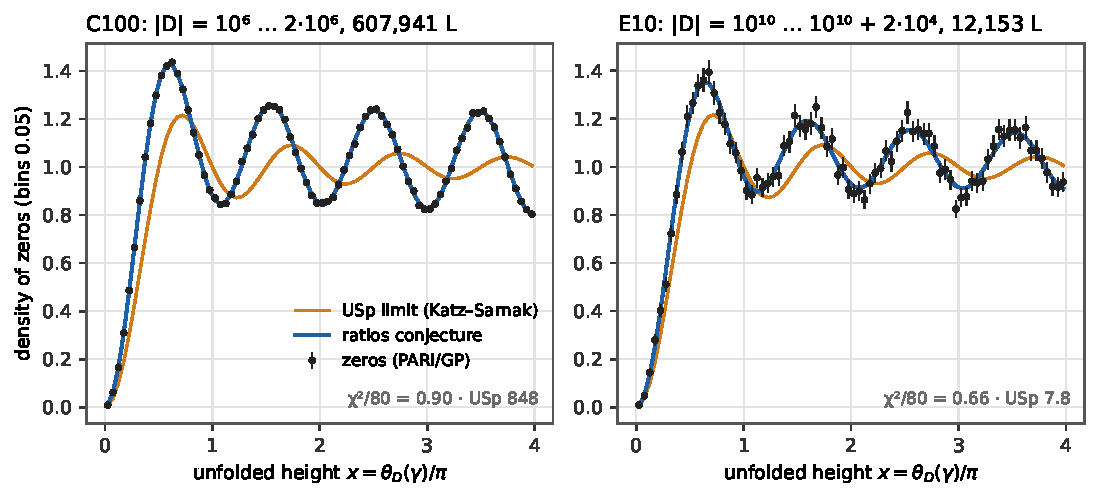
\includegraphics[width=0.95\textwidth,height=\textheight]{../figures/01_density_en.pdf}
\caption{Figure 1. Density of the unfolded zeros in bins of 0.05 for the
families C100 (left) and E10 (right) against the ratios conjecture
(blue) and the Katz--Sarnak limit USp (orange).}
\end{figure}

{\small\begin{longtable}[]{@{}
  >{\raggedright\arraybackslash}p{(\columnwidth - 8\tabcolsep) * \real{0.0896}}
  >{\raggedleft\arraybackslash}p{(\columnwidth - 8\tabcolsep) * \real{0.1194}}
  >{\raggedright\arraybackslash}p{(\columnwidth - 8\tabcolsep) * \real{0.2687}}
  >{\raggedleft\arraybackslash}p{(\columnwidth - 8\tabcolsep) * \real{0.1642}}
  >{\raggedright\arraybackslash}p{(\columnwidth - 8\tabcolsep) * \real{0.3582}}@{}}
\toprule\noalign{}
\begin{minipage}[b]{\linewidth}\raggedright
family
\end{minipage} & \begin{minipage}[b]{\linewidth}\raggedleft
\(\ln|D|\)
\end{minipage} & \begin{minipage}[b]{\linewidth}\raggedright
\(\chi^2\)/bin 0.05: ratios / without \(A\) / USp
\end{minipage} & \begin{minipage}[b]{\linewidth}\raggedleft
\(p\) (bootstrap)
\end{minipage} & \begin{minipage}[b]{\linewidth}\raggedright
density in \([0, \frac12]\): data / ratios / USp
\end{minipage} \\
\midrule\noalign{}
\endhead
\bottomrule\noalign{}
\endlastfoot
A & 7.55 & 0.57 / 2.0 / 8.3 & \textless{} 0.005 & \(0.772 \pm 0.036\) /
0.771 / 0.411 \\ \addlinespace[2pt]
B & 9.60 & 0.54 / 5.0 / 21 & \textless{} 0.005 & \(0.708 \pm 0.015\) /
0.702 / 0.411 \\ \addlinespace[2pt]
B10 & 10.77 & 0.87 / 33 / 142 & 0.34 & \(0.6718 \pm 0.0050\) / 0.6729 /
0.411 \\ \addlinespace[2pt]
C10 & 13.86 & 1.06 / 22 / 89 & 0.78 & \(0.6136 \pm 0.0045\) / 0.6134 /
0.411 \\ \addlinespace[2pt]
C100 & 14.20 & 0.90 / 203 / 848 & 0.34 & \(0.6082 \pm 0.0014\) / 0.6084
/ 0.411 \\ \addlinespace[2pt]
D10 & 18.42 & 0.98 / 1.8 / 5.1 & 0.60 & \(0.558 \pm 0.014\) / 0.560 /
0.411 \\ \addlinespace[2pt]
D100 & 18.42 & 0.77 / 12 / 49 & 0.10 & \(0.5591 \pm 0.0043\) / 0.5595 /
0.411 \\ \addlinespace[2pt]
E & 23.03 & 0.71 / 0.80 / 1.2 & 0.04 & \(0.531 \pm 0.030\) / 0.527 /
0.411 \\ \addlinespace[2pt]
E10 & 23.03 & 0.66 / 2.6 / 7.8 & 0.02 & \(0.5273 \pm 0.0093\) / 0.5267 /
0.411 \\ \addlinespace[2pt]
R & 15.38 & 1.19 / 3.1 / 8.5 & 0.93 & \(0.609 \pm 0.014\) / 0.593 /
0.411 \\ \addlinespace[2pt]
R10 & 15.37 & 0.90 / 18 / 72 & 0.37 & \(0.5933 \pm 0.0044\) / 0.5925 /
0.411 \\ \addlinespace[2pt]
\end{longtable}}

The ratios conjecture describes every family (Figure 1, Figure 2):
\(\chi^2\) per bin 0.54--1.19 at bin width 0.05, where independent
L-functions around an exact model give 0.95 and the bootstrap band is
0.70--1.24; the null models give up to 203 (without the arithmetic
factor) and 848 (USp) in the largest family. The density in
\([0, \frac12]\) agrees with the conjecture in all 33 combinations of
family and sign within 1.2 standard errors; in C100 the error is 0.0014.
The number of zeros up to \(x = 4\) per L-function agrees as well (C100:
4.0103 against 4.0105; the USp limit gives 3.756). The same holds at the
bin widths 0.025 and 0.1 and without bins (data files). Several families
have \(\chi^2\) below 0.95 --- Section 4.3.

\begin{figure}
\centering
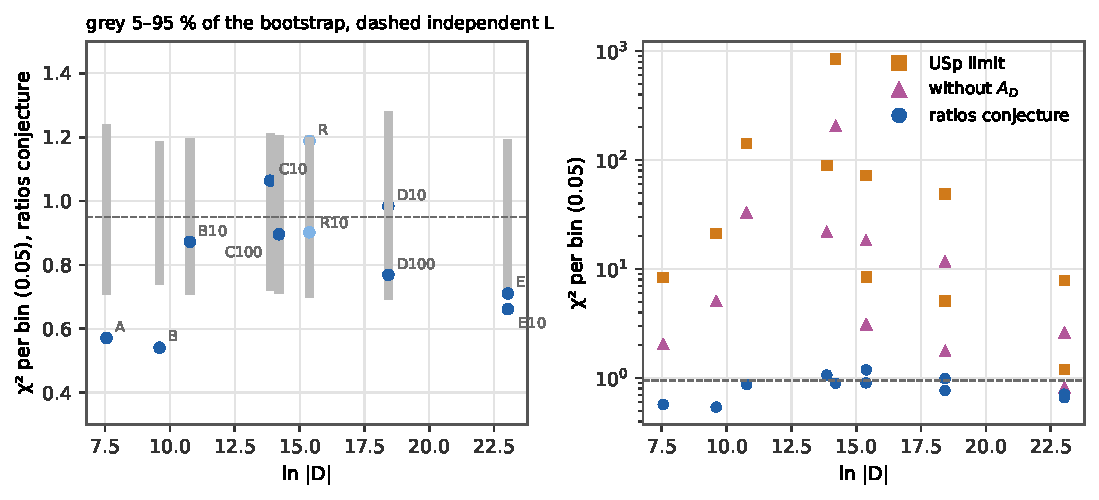
\includegraphics[width=0.95\textwidth,height=\textheight]{../figures/02_chi2_families_en.pdf}
\caption{Figure 2. Left: \(\chi^2\) per bin (0.05) of the ratios
conjecture for all families against \(\ln|D|\) with the 5--95 \% band of
the bootstrap (grey) and the expectation for independent L-functions
(dashed); random families in light blue. Right: the same for the USp
limit and for the model without the arithmetic factor (log scale).}
\end{figure}

\hypertarget{the-approach-to-the-katzsarnak-limit}{%
\subsection{4.2 The approach to the Katz--Sarnak
limit}\label{the-approach-to-the-katzsarnak-limit}}

\begin{figure}
\centering
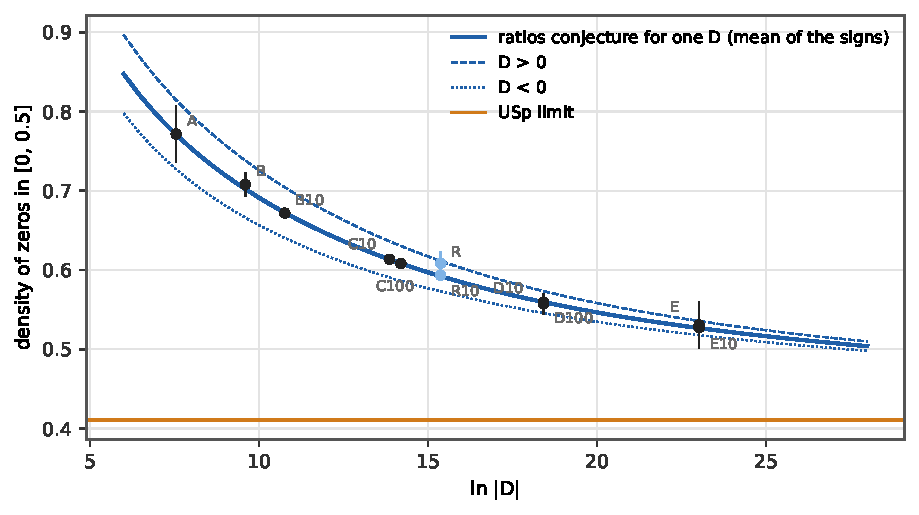
\includegraphics[width=0.8\textwidth,height=\textheight]{../figures/03_approach_en.pdf}
\caption{Figure 3. Density of the zeros in \([0, \frac12]\) against
\(\ln|D|\): families (points), the ratios conjecture for one
discriminant (lines; mean of the signs, \(D > 0\) dashed, \(D < 0\)
dotted) and the USp limit 0.411; random families light blue.}
\end{figure}

The density near the central point decreases from 0.772 at
\(|D| \approx 2\cdot10^3\) to 0.527 at \(10^{10}\) and follows the
ratios conjecture for one discriminant (Figure 3), which reaches the USp
value 0.411 only slowly (0.504 at \(\ln|D| = 28\)). At \(|D| = 10^{10}\)
the data are \(0.5273 \pm 0.0093\) --- 12.6 standard errors above the
limit. The limit of Katz and Sarnak is not in sight at these conductors;
the lower-order terms of the ratios conjecture are.

\hypertarget{why-consecutive-families-give-chi2-below-0.95}{%
\subsection{\texorpdfstring{4.3 Why consecutive families give \(\chi^2\)
below
0.95}{4.3 Why consecutive families give \textbackslash chi\^{}2 below 0.95}}\label{why-consecutive-families-give-chi2-below-0.95}}

The families A, B, E and E10 have \(\chi^2\) per bin well below 0.95
(bootstrap probability below 0.005 for A and B, 0.035 and 0.02 for E and
E10); B was the clearest case, 0.54 at bin width 0.05 and 0.45 at 0.1
(0.85 at 0.025), and below 0.65 for each sign. The deficit is largest
for the widest bins --- a first hint at low frequencies. The random
families R and R10 are not below. To find out whether this is a property
of consecutive discriminants, B10, C100 and D100 were split into bands
of 6,074 consecutive discriminants and compared with samples of the same
size (Figure 4).

\begin{figure}
\centering
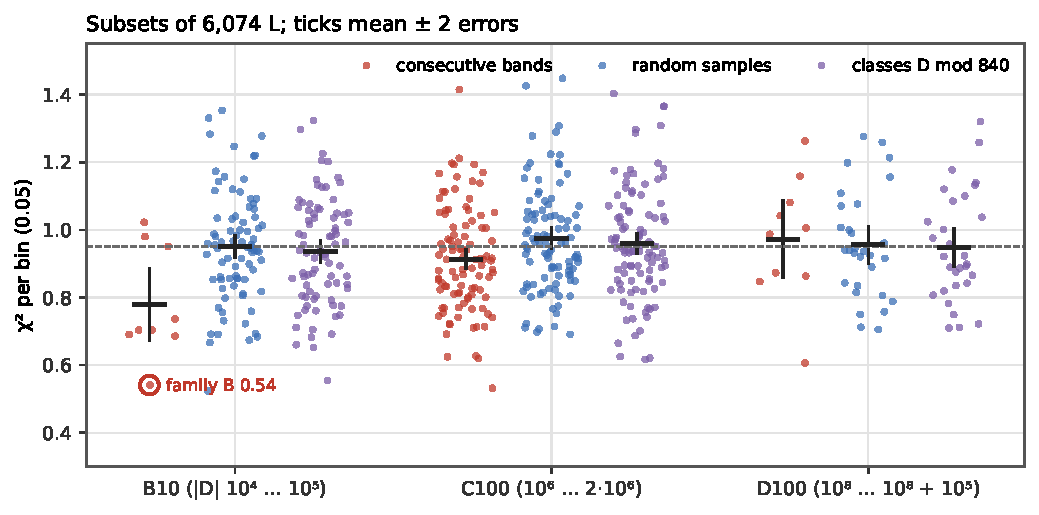
\includegraphics[width=0.95\textwidth,height=\textheight]{../figures/04_subsets_en.pdf}
\caption{Figure 4. \(\chi^2\) per bin of subsets of 6,074 L-functions:
consecutive bands (red), random samples (blue) and random samples with
the classes \(D \bmod 840\) of the whole family (violet); ticks mean
\(\pm\) 2 errors. The ring marks family B, the first band of B10.}
\end{figure}

{\small\begin{longtable}[]{@{}
  >{\raggedright\arraybackslash}p{(\columnwidth - 10\tabcolsep) * \real{0.0811}}
  >{\raggedright\arraybackslash}p{(\columnwidth - 10\tabcolsep) * \real{0.1892}}
  >{\raggedright\arraybackslash}p{(\columnwidth - 10\tabcolsep) * \real{0.1757}}
  >{\raggedright\arraybackslash}p{(\columnwidth - 10\tabcolsep) * \real{0.1757}}
  >{\raggedright\arraybackslash}p{(\columnwidth - 10\tabcolsep) * \real{0.1892}}
  >{\raggedright\arraybackslash}p{(\columnwidth - 10\tabcolsep) * \real{0.1892}}@{}}
\toprule\noalign{}
\begin{minipage}[b]{\linewidth}\raggedright
family
\end{minipage} & \begin{minipage}[b]{\linewidth}\raggedright
subsets
\end{minipage} & \begin{minipage}[b]{\linewidth}\raggedright
\(\chi^2\)/bin 0.05
\end{minipage} & \begin{minipage}[b]{\linewidth}\raggedright
\(\chi^2\)/bin 0.1
\end{minipage} & \begin{minipage}[b]{\linewidth}\raggedright
power at \(k = 1 \dots 7\)
\end{minipage} & \begin{minipage}[b]{\linewidth}\raggedright
power at \(k = 32 \dots 79\)
\end{minipage} \\
\midrule\noalign{}
\endhead
\bottomrule\noalign{}
\endlastfoot
B10 & 9 bands & \(0.779 \pm 0.055\) & \(0.686 \pm 0.058\) &
\(0.0098 \pm 0.0048\) & \(0.540 \pm 0.049\) \\ \addlinespace[2pt]
& 81 random & \(0.951 \pm 0.018\) & \(0.861 \pm 0.023\) &
\(0.0433 \pm 0.0031\) & \(0.622 \pm 0.016\) \\ \addlinespace[2pt]
& 81 with classes mod 840 & \(0.936 \pm 0.018\) & \(0.816 \pm 0.020\) &
\(0.0365 \pm 0.0030\) & \(0.633 \pm 0.015\) \\ \addlinespace[2pt]
C100 & 100 bands & \(0.913 \pm 0.015\) & \(0.801 \pm 0.020\) &
\(0.0187 \pm 0.0014\) & \(0.609 \pm 0.013\) \\ \addlinespace[2pt]
& 100 random & \(0.976 \pm 0.017\) & \(0.930 \pm 0.022\) &
\(0.0518 \pm 0.0029\) & \(0.623 \pm 0.012\) \\ \addlinespace[2pt]
& 100 with classes mod 840 & \(0.960 \pm 0.017\) & \(0.897 \pm 0.021\) &
\(0.0447 \pm 0.0027\) & \(0.604 \pm 0.012\) \\ \addlinespace[2pt]
D100 & 10 bands & \(0.973 \pm 0.059\) & \(0.888 \pm 0.068\) &
\(0.0246 \pm 0.0034\) & \(0.635 \pm 0.045\) \\ \addlinespace[2pt]
& 30 random & \(0.956 \pm 0.029\) & \(0.907 \pm 0.040\) &
\(0.0517 \pm 0.0054\) & \(0.601 \pm 0.025\) \\ \addlinespace[2pt]
& 30 with classes mod 840 & \(0.949 \pm 0.030\) & \(0.905 \pm 0.034\) &
\(0.0443 \pm 0.0059\) & \(0.610 \pm 0.030\) \\ \addlinespace[2pt]
\end{longtable}}

In B10 and C100 the consecutive bands are below the random samples by
3.0 and 2.8 standard errors in \(\chi^2\); in D100 there is no
difference in \(\chi^2\). The cosine decomposition shows where the
difference sits (Figure 5): at low frequencies, \(k = 1 \dots 7\) or
\(u < 1\), the bands have 0.23, 0.36 and 0.48 of the power of the random
samples in B10, C100 and D100 (5.9, 10.2 and 4.3 standard errors), at
high frequencies \(k = 32 \dots 79\) there is no significant difference
(\(-1.6\), \(-0.8\) and \(+0.7\) standard errors). The total \(\chi^2\)
shows the effect only where the suppressed low frequencies are a large
enough share of it.

\begin{figure}
\centering
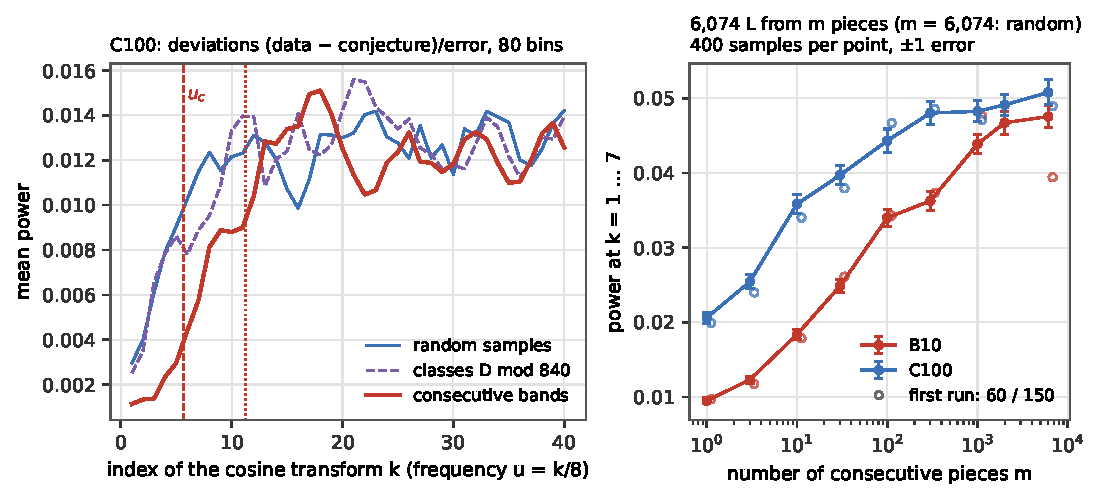
\includegraphics[width=0.95\textwidth,height=\textheight]{../figures/05_spectrum_pieces_en.pdf}
\caption{Figure 5. Left: mean power of the cosine transform of the
deviations in C100 for consecutive bands (red), random samples (blue)
and samples with the classes mod 840 (violet, dashed), as a running mean
over three neighbouring \(k\); vertical lines \(u_c\) and \(2u_c\).
Right: power at \(k = 1 \dots 7\) of subsets assembled from \(m\)
consecutive pieces at random positions, 400 subsets per point with
\(\pm 1\) error (filled); open circles the first run with 60 (B10) and
150 (C100) subsets per point, shifted slightly to the right --- its
apparent peak of B10 at \(m = 1\,000\) is the scatter of a small number
of random subsets.}
\end{figure}

\textbf{Mechanism.} By the explicit formula, the deviation of the
one-level density of a set \(\mathcal S\) of discriminants from its mean
contains, for every prime \(p\), a term proportional to
\(\frac{\ln p}{\sqrt p}\langle\chi_D(p)\rangle_{\mathcal S}\cos(t\ln p)\),
and from the prime squares a term with
\(\langle\chi_D(p)^2\rangle_{\mathcal S}\) and \(\cos(2t\ln p)\). In the
unfolded variable \(t\ln p = 2\pi x\,\ln p/l\) (to leading order), so
the prime \(p\) acts at the frequency \(u = \ln p/l\). For a stretch of
consecutive discriminants of length \(\Delta\) (in \(|D|\)),
\(\chi_D(p)\) depends on \(D\) only modulo \(p\) (modulo 8 for
\(p = 2\)), and for \(p < \Delta\) the average runs over nearly complete
periods: it is of order \(p/N\) instead of \(N^{-1/2}\) for a random
sample of \(N\) discriminants; the same holds for the proportion of
\(D\) divisible by \(p\). The fluctuations of the family density are
therefore suppressed below \(u_c = \ln\Delta/l\) (from \(\chi_D(p)\))
and partly up to \(2u_c\) (from the prime squares). For bands of 6,074
discriminants \(\Delta \approx 10^4\), and \(u_c = 0.96\), 0.71 and 0.53
in B10, C100 and D100 --- the suppressed range shrinks with the
conductor, as observed. The periodicity of \(\chi_d(n)\) in \(d\) is the
standard tool of mean-value theorems over discriminants {[}14, 15{]}.
The closest published measurement is the murmuration of quadratic
characters {[}16{]}: the average of \(\chi_{8d}(p)\) over \(d\) near
\(X\) depends only on \(p/X\), tends to 0 as \(p/X \to 0\) and changes
near \(p \approx X\), which the authors link to the transition at
support 1 of the one-level density of a symplectic family {[}7, 17{]}.
In this language \(u_c = \ln\Delta/l\) is that transition for a family
of length \(\Delta\) instead of \(X\) (our interpretation; made more
formal in Section 4.6). Two tests, with a caution on random sampling:

\begin{itemize}
\tightlist
\item
  \emph{Pieces.} A subset made of \(m\) consecutive pieces of length
  \(\Delta/m\) has \(u_c = \ln(\Delta/m)/l\): the shorter the pieces,
  the fewer primes run over complete periods inside a piece. With 400
  subsets per point the power at \(k = 1 \dots 7\) grows with \(m\) from
  0.0095 ± 0.0004 (\(m = 1\)) to 0.0476 ± 0.0014 (random sample) in B10
  and from 0.0206 ± 0.0008 to 0.0508 ± 0.0017 in C100, monotonically
  within the errors (Spearman rank correlation with \(\ln m\) 1.00 in
  both; Figure 5, right); an independent repetition with other random
  positions gives the same. B10 reaches the random value later than C100
  because the same piece has a higher limit \(u_c\) at the smaller
  conductor (\(l\) = 9.6 against 13.1; at \(m = 300\), \(u_c\) = 0.36
  against 0.27), so the suppression reaches further into the low modes.
  At \(m = 1\,000\) a small suppression probably remains in B10 (0.0428
  ± 0.0004 against 0.0452 ± 0.0012 for random samples, means of four
  independent runs): a piece of about six discriminants still covers
  whole periods of \(p = 2, 3, 5\).
\item
  \emph{Random sampling.} Every point is a mean over random subsets, and
  its error is the standard deviation of the subsets divided by the
  square root of their number. The power of a single subset scatters by
  60--90 \% of its mean (it is a sum of seven squared cosine
  coefficients), so with 60 subsets the error of a point is about a
  tenth of its value. The first run of this test, with 60 subsets per
  point in B10 and 150 in C100 (open circles in Figure 5), showed in B10
  an apparent peak at \(m = 1\,000\) (0.0477 ± 0.0046) followed by a
  drop to the random sample (0.0394 ± 0.0027), a fall of 1.5 joint
  errors between two neighbouring points. With 400 subsets per point the
  peak is gone (0.0439 ± 0.0013 and 0.0476 ± 0.0014), and four
  independent runs of 400 subsets give 0.0419--0.0439 at \(m = 1\,000\)
  and 0.0421--0.0476 for random samples. A step between neighbouring
  points of a curve built from random samples is therefore a finding
  only when it is large compared with the errors of both points, and the
  random value of B10 is quoted as a mean with its error, not as a
  single run.
\item
  \emph{Residue classes.} Random samples with the composition of the
  whole family in the classes (sign, \(D \bmod 840\)) fix the averages
  of \(\chi_D(p)\) only for \(p = 2, 3, 5, 7\); they lower the
  low-frequency power by only 14--16 \% (a fifth to a quarter of the
  deficit of the bands) and leave \(\chi^2\) where the random samples
  are (Table). The effect is carried by the whole range of primes up to
  the length of the stretch, not by the smallest primes. Section 4.4
  tests 19 moduli and the sign; with four to five times more samples
  there the reduction by \(D \bmod 840\) is 18 \% in B10 (\(z = -5.1\))
  and not significant in C100 and D100.
\end{itemize}

\textbf{Family B.} In B10 the nine bands from \(|D| = 10^4\) give
\(\chi^2\) = 0.54, 0.69, 0.69, 0.74, 0.70, 0.98, 0.95, 1.02, 0.70; the
first is family B. It is the lowest band, 1.5 standard deviations below
their mean 0.78: the general effect of consecutiveness at a small
conductor plus an ordinary fluctuation. For the whole family B10
(\(\Delta = 9\cdot10^4\)) the suppressed share is smaller relative to
the bootstrap band, and \(\chi^2 = 0.87\) (probability 0.34). The effect
is a property of how the family is chosen, not of the zeros of single
L-functions: the random families, which sample the same range of
conductors, show none.

\hypertarget{residue-classes-for-19-moduli-and-the-sums-of-characters}{%
\subsection{4.4 Residue classes for 19 moduli and the sums of
characters}\label{residue-classes-for-19-moduli-and-the-sums-of-characters}}

Section 4.3 tested one stratification, (sign, \(D \bmod 840\)). To see
whether any modulus reproduces the effect of consecutive bands, the test
was repeated for 19 moduli --- the primes and prime powers 3, 5, 7, 8,
9, 13, 16, 41 and 131 and the composite moduli 24, 40, 120, 130, 260,
360, 369, 520, 800 and 840 --- and for the sign of \(D\) alone
(\(M = 1\)). All subsets of this section are new draws, independent of
those of Section 4.3: a first pass with 81 / 100 / 30 samples per
stratification and an independent repetition with other seeds and more
samples (300 / 300 / 100 in B10 / C100 / D100) was made for the random
samples, the sign and the moduli 3, 7, 8, 16, 41, 360, 520 and 840, and
the prime 131 was added in a separate run of the same size.

{\small\begin{longtable}[]{@{}
  >{\raggedright\arraybackslash}p{(\columnwidth - 8\tabcolsep) * \real{0.2000}}
  >{\raggedright\arraybackslash}p{(\columnwidth - 8\tabcolsep) * \real{0.2000}}
  >{\raggedright\arraybackslash}p{(\columnwidth - 8\tabcolsep) * \real{0.2000}}
  >{\raggedright\arraybackslash}p{(\columnwidth - 8\tabcolsep) * \real{0.2000}}
  >{\raggedright\arraybackslash}p{(\columnwidth - 8\tabcolsep) * \real{0.2000}}@{}}
\toprule\noalign{}
\begin{minipage}[b]{\linewidth}\raggedright
stratification
\end{minipage} & \begin{minipage}[b]{\linewidth}\raggedright
\(W_{100}\) (B10 / C100 / D100)
\end{minipage} & \begin{minipage}[b]{\linewidth}\raggedright
B10
\end{minipage} & \begin{minipage}[b]{\linewidth}\raggedright
C100
\end{minipage} & \begin{minipage}[b]{\linewidth}\raggedright
D100
\end{minipage} \\
\midrule\noalign{}
\endhead
\bottomrule\noalign{}
\endlastfoot
random & 1 / 1 / 1 & 0.0440 & 0.0489 & 0.0499 \\ \addlinespace[2pt]
consecutive bands & 0.04 / 0.04 / 0.05 & 0.0098 (\(-7.0\)) & 0.0187
(\(-16.2\)) & 0.0246 (\(-6.4\)) \\ \addlinespace[2pt]
sign only & 1.00 / 1.00 / 1.00 & 0.0452 (\(+0.6\)) & 0.0490 (\(+0.0\)) &
0.0497 (\(-0.0\)) \\ \addlinespace[2pt]
\(D \bmod 3\) & 0.96 / 0.96 / 0.96 & 0.0468 (\(+1.5\)) & 0.0508
(\(+0.9\)) & 0.0480 (\(-0.6\)) \\ \addlinespace[2pt]
\(D \bmod 5\) & 0.95 / 0.95 / 0.95 & 0.0479 (\(+1.0\)) & 0.0510
(\(+0.6\)) & 0.0573 (\(+1.3\)) \\ \addlinespace[2pt]
\(D \bmod 7\) & 0.94 / 0.94 / 0.94 & 0.0436 (\(-0.2\)) & 0.0508
(\(+0.9\)) & 0.0487 (\(-0.3\)) \\ \addlinespace[2pt]
\(D \bmod 8\) & 0.98 / 0.98 / 0.98 & 0.0414 (\(-1.5\)) & 0.0480
(\(-0.5\)) & 0.0457 (\(-1.4\)) \\ \addlinespace[2pt]
\(D \bmod 9\) & 0.96 / 0.96 / 0.96 & 0.0424 (\(-0.5\)) & 0.0493
(\(+0.1\)) & 0.0552 (\(+0.9\)) \\ \addlinespace[2pt]
\(D \bmod 13\) & 0.94 / 0.94 / 0.94 & 0.0442 (\(+0.1\)) & 0.0485
(\(-0.1\)) & 0.0512 (\(+0.2\)) \\ \addlinespace[2pt]
\(D \bmod 16\) & 0.98 / 0.98 / 0.98 & 0.0425 (\(-0.9\)) & 0.0518
(\(+1.4\)) & 0.0478 (\(-0.6\)) \\ \addlinespace[2pt]
\(D \bmod 24\) & 0.94 / 0.94 / 0.94 & 0.0431 (\(-0.3\)) & 0.0503
(\(+0.4\)) & 0.0425 (\(-1.4\)) \\ \addlinespace[2pt]
\(D \bmod 40\) & 0.93 / 0.93 / 0.93 & 0.0390 (\(-1.7\)) & 0.0464
(\(-0.7\)) & 0.0422 (\(-1.4\)) \\ \addlinespace[2pt]
\(D \bmod 41\) & 0.96 / 0.96 / 0.96 & 0.0445 (\(+0.3\)) & 0.0505
(\(+0.8\)) & 0.0438 (\(-2.0\)) \\ \addlinespace[2pt]
\(D \bmod 120\) & 0.89 / 0.89 / 0.89 & 0.0420 (\(-0.7\)) & 0.0506
(\(+0.5\)) & 0.0555 (\(+0.9\)) \\ \addlinespace[2pt]
\(D \bmod 130\) & 0.89 / 0.89 / 0.89 & 0.0460 (\(+0.6\)) & 0.0531
(\(+1.4\)) & 0.0508 (\(+0.2\)) \\ \addlinespace[2pt]
\(D \bmod 131\) & 1.00 / 1.00 / 1.00 & 0.0451 (\(+0.6\)) & 0.0505
(\(+0.7\)) & 0.0547 (\(+1.2\)) \\ \addlinespace[2pt]
\(D \bmod 260\) & 0.89 / 0.89 / 0.89 & 0.0447 (\(+0.2\)) & 0.0526
(\(+1.0\)) & 0.0485 (\(-0.2\)) \\ \addlinespace[2pt]
\(D \bmod 360\) & 0.90 / 0.89 / 0.89 & 0.0402 (\(-2.1\)) & 0.0468
(\(-1.1\)) & 0.0456 (\(-1.3\)) \\ \addlinespace[2pt]
\(D \bmod 369\) & 0.93 / 0.92 / 0.93 & 0.0434 (\(-0.2\)) & 0.0551
(\(+1.7\)) & 0.0511 (\(+0.3\)) \\ \addlinespace[2pt]
\(D \bmod 520\) & 0.88 / 0.87 / 0.88 & 0.0425 (\(-0.8\)) & 0.0476
(\(-0.7\)) & 0.0479 (\(-0.6\)) \\ \addlinespace[2pt]
\(D \bmod 800\) & 0.94 / 0.93 / 0.94 & 0.0415 (\(-0.8\)) & 0.0479
(\(-0.3\)) & 0.0395 (\(-2.4\)) \\ \addlinespace[2pt]
\(D \bmod 840\) & 0.84 / 0.83 / 0.84 & 0.0359 (\(-5.1\)) & 0.0462
(\(-1.4\)) & 0.0518 (\(+0.6\)) \\ \addlinespace[2pt]
\end{longtable}}

Power of the cosine coefficients \(k = 1 \dots 7\) of subsets of 6,074
L-functions, mean over 81--681 (B10), 100--700 (C100) and 30--230 (D100)
samples (all runs together; consecutive bands 9 / 100 / 10), in brackets
\(z\) = (stratification \(-\) random) / joint error. \(W_{100}\) is the
exact remaining share of stratified sampling without replacement
(Section 3), for all stratifications.

In C100 and D100 no stratification differs from the random samples
beyond what 40 tests give by chance: beyond 2 standard errors are only
D100 mod 800 (\(z = -2.4\), 30 samples) and mod 41 (\(-2.0\)). In B10
the only clear reduction is \(D \bmod 840\) (\(z = -5.1\)), followed by
360 (\(-2.1\)). Balancing \(D \bmod 8\) or \(D \bmod 16\), which fixes
\(\chi_D(2)\), is not decisive (\(z = -1.5 / -0.5 / -1.4\) and
\(-0.9 / +1.4 / -0.6\)), and the sign alone does nothing. A first run
with 30 samples gave \(0.0606 \pm 0.0073\) for D100 mod 840; with the
repetition (130 samples) the value is \(0.0518 \pm 0.0028\), as for
random samples.

\textbf{Character sums without zeros.} Random samples have the variance
of the means of \(\chi_D(p)\) of sampling from a finite population
within 0.4 \% (median ratio 1.0011 / 1.0022 / 0.9960 over 300 draws).
For a stratification by \(M\) the exact variance of stratified sampling
without replacement is at most 0.07 of the random value for the primes
dividing \(M\) (for \(p = 2\) only when \(8 \mid M\); the remainder is
the rounding of the class counts) and 1.000--1.014 for every other
prime. The share \(W_{100}\) that a stratified subset keeps is therefore
at least 0.83 for every one of the 20 stratifications (0.84 / 0.83 /
0.84 for 840; Table), against 0.04--0.05 for consecutive bands. The line
through the two points of each family --- random samples (\(W = 1\)) and
consecutive bands --- gives for all 60 stratified subsets
\(\chi^2 = 82.05\) with the covariance of the two shared points
(\(p = 0.03\); the central 95 \% range for 60 degrees of freedom is
40.5--83.3), and for the 33 of the first version of this section
\(\chi^2 = 47.7\) (\(p = 0.05\)). The direction agrees: no
stratification comes near the bands (Figure 6, left). The size agrees
only at the edge: 42 of the 60 deviations are positive (mean
\(z = +0.56\)), the stratifications lower the low-frequency power of the
zeros a little less than the line predicts. A likely reason is that the
line attributes the whole deficit of the bands to the primes up to 100,
while the bands also suppress the primes between 100 and \(10^4\)
(profile below), which a modulus does not touch. Two checks: the slope
fitted to the 20 stratifications alone, divided by the slope of the
line, gives the share of the band deficit carried by \(p \le 100\) as
1.09 ± 0.26, 0.53 ± 0.26 and 0.02 ± 0.54 in B10, C100 and D100 (jointly
0.72 ± 0.17) --- it falls with the conductor, as the low modes are
carried by ever larger primes, but only at the level of 1.5--2 errors;
and equal weights \((\ln p)^2/p\) over all primes of the low modes
(\(W_E\), bands 0.18 / 0.53 / 0.75) remove the shift (mean
\(z = +0.02\)) but overshoot in B10 (\(\chi^2 = 91.0\), \(p = 0.006\),
B10 mod 840 4.1 errors below). The two axes come from different data ---
the zeros on one side, the values of the characters on the other --- so
the agreement in direction is an independent check of the mechanism of
Section 4.3: a modulus fixes only the primes that divide it, while the
low frequencies are carried by all primes up to the thousands; how the
variance of \(\chi_D(p)\) converts into low-frequency power is
understood in direction, not in size.

\begin{figure}
\centering
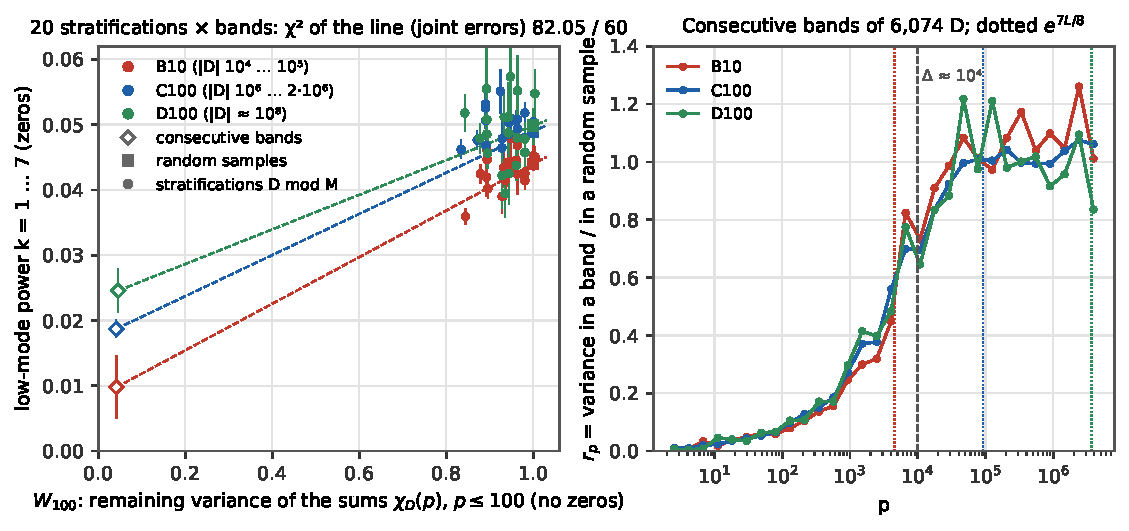
\includegraphics[width=0.95\textwidth,height=\textheight]{../figures/06_moduli_characters_en.pdf}
\caption{Figure 6. Left: exact remaining share \(W_{100}\) of the
weighted variance of the means of \(\chi_D(p)\), \(p \le 100\) (from the
characters, without zeros), against the low-frequency power
\(k = 1 \dots 7\) of the zeros (from the zeros, without characters) for
random samples (squares), the 20 stratifications (dots) and consecutive
bands (diamonds) of B10, C100 and D100, with \(\pm 1\) error; dashed the
line through the two points of each family. Right: profile \(r_p\) of
consecutive bands of 6,074 discriminants (582 primes up to
\(4\cdot10^6\) in logarithmic bins); dashed the width
\(\Delta \approx 10^4\) of a band, dotted \(e^{7L/8}\) for each family.}
\end{figure}

\textbf{Conductor dependence.} The profile \(r_p\) of consecutive bands
is the same function of \(p\) in the three families, whose bands all
have the width \(\Delta \approx 10^4\) in \(|D|\): 0.04--0.05 for
\(p \le 100\), 0.12--0.17 up to \(10^3\), 0.29--0.41 up to \(10^4\),
0.84--0.90 up to \(10^5\) and about 1 above (Figure 6, right). The mode
\(k\) is carried by primes with \(\ln p \approx kL/8\),
\(L = \ln(|D|/\pi)\), i.e.~up to \(e^{7L/8} \approx 4\cdot10^3\),
\(9\cdot10^4\) and \(4\cdot10^6\) in B10, C100 and D100; the
\(k\)-weighted share \(W_k = \sum_k k\,r(e^{kL/8})/28\) grows
\(0.22 \to 0.61 \to 0.70\), while the measured ratio of the
low-frequency power of bands and random samples grows
\(0.22 \pm 0.11 \to 0.38 \pm 0.03 \to 0.49 \pm 0.07\). Order and
direction agree; the size for C100 does not (7 errors). The conversion
of the variance of \(\chi_D(p)\) into the low-frequency power of
consecutive bands is thus understood in its direction but not in its
size.

\hypertarget{the-first-zero}{%
\subsection{4.5 The first zero}\label{the-first-zero}}

\begin{figure}
\centering
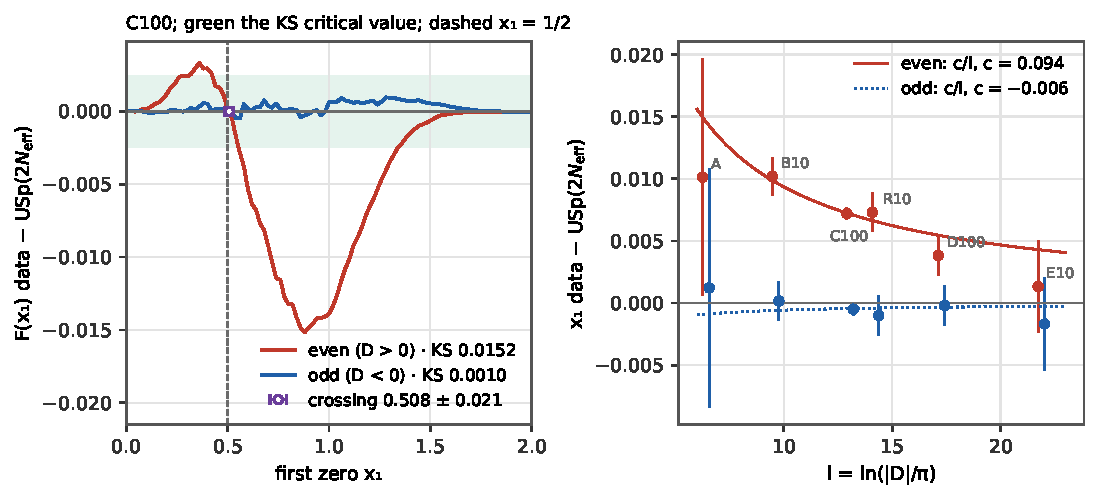
\includegraphics[width=0.95\textwidth,height=\textheight]{../figures/07_first_zero_en.pdf}
\caption{Figure 7. Left: distribution function of the first zero in C100
minus USp\((2N_{\mathrm{eff}})\) for even (red) and odd (blue)
characters; green the Kolmogorov--Smirnov critical value, dashed
\(x_1 = \frac12\) (the end of the interval on which \(N_{\mathrm{eff}}\)
is fixed), violet the crossing of the even curve with zero with its
error (grid 0.001, bootstrap). Right: deviation of the mean first zero
from USp\((2N_{\mathrm{eff}})\) against \(l = \ln(|D|/\pi)\) in six
non-overlapping families, with the fits \(c/l\).}
\end{figure}

USp\((2N)\) with \(N = \frac12\ln(|D|/\pi)\) does not describe the first
zero: its mean is 0.67--0.75 against the measured 0.58--0.70, and the
Kolmogorov--Smirnov distance is 0.06--0.14, 1.6 to 53 times the critical
value. The effective \(N_{\mathrm{eff}}\) fixed by the ratios conjecture
is 1.5--4.5, two to three times smaller than \(\frac12 l\), and
USp\((2N_{\mathrm{eff}})\) gives the mean first zero within 1.1 \% in
all families. Separating the signs with the errors of C100, B10, D100,
E10 and R10 shows a difference (Figure 7):

{\small\begin{longtable}[]{@{}
  >{\raggedright\arraybackslash}p{(\columnwidth - 10\tabcolsep) * \real{0.0822}}
  >{\raggedleft\arraybackslash}p{(\columnwidth - 10\tabcolsep) * \real{0.0959}}
  >{\raggedright\arraybackslash}p{(\columnwidth - 10\tabcolsep) * \real{0.2466}}
  >{\raggedright\arraybackslash}p{(\columnwidth - 10\tabcolsep) * \real{0.1644}}
  >{\raggedright\arraybackslash}p{(\columnwidth - 10\tabcolsep) * \real{0.2466}}
  >{\raggedright\arraybackslash}p{(\columnwidth - 10\tabcolsep) * \real{0.1644}}@{}}
\toprule\noalign{}
\begin{minipage}[b]{\linewidth}\raggedright
family
\end{minipage} & \begin{minipage}[b]{\linewidth}\raggedleft
\(l\)
\end{minipage} & \begin{minipage}[b]{\linewidth}\raggedright
even (\(D > 0\)): \(x_1 - x_1^{\mathrm{eff}}\)
\end{minipage} & \begin{minipage}[b]{\linewidth}\raggedright
KS / critical
\end{minipage} & \begin{minipage}[b]{\linewidth}\raggedright
odd (\(D < 0\)): \(x_1 - x_1^{\mathrm{eff}}\)
\end{minipage} & \begin{minipage}[b]{\linewidth}\raggedright
KS / critical
\end{minipage} \\
\midrule\noalign{}
\endhead
\bottomrule\noalign{}
\endlastfoot
A & 6.41 & \(+0.0101 \pm 0.0095\) & 0.032 / 0.055 &
\(+0.0012 \pm 0.0096\) & 0.017 / 0.055 \\ \addlinespace[2pt]
B10 & 9.62 & \(+0.0102 \pm 0.0015\) & 0.025 / 0.008 &
\(+0.0002 \pm 0.0015\) & 0.003 / 0.008 \\ \addlinespace[2pt]
C100 & 13.06 & \(+0.0072 \pm 0.0005\) & 0.015 / 0.0025 &
\(-0.0005 \pm 0.0005\) & 0.0010 / 0.0025 \\ \addlinespace[2pt]
R10 & 14.23 & \(+0.0073 \pm 0.0016\) & 0.014 / 0.008 &
\(-0.0010 \pm 0.0016\) & 0.003 / 0.008 \\ \addlinespace[2pt]
D100 & 17.28 & \(+0.0038 \pm 0.0016\) & 0.008 / 0.008 &
\(-0.0002 \pm 0.0016\) & 0.003 / 0.008 \\ \addlinespace[2pt]
E10 & 21.88 & \(+0.0013 \pm 0.0037\) & 0.006 / 0.017 &
\(-0.0017 \pm 0.0037\) & 0.006 / 0.018 \\ \addlinespace[2pt]
\end{longtable}}

For odd characters USp\((2N_{\mathrm{eff}})\) gives the whole
distribution of the first zero within the errors at every conductor from
\(10^3\) to \(10^{10}\) (in C100 the Kolmogorov--Smirnov distance is
0.0010 at the critical value 0.0025); the fit \(c/l\) gives
\(c = -0.006 \pm 0.006\). For even characters the first zero lies
higher: 14.8 standard errors in C100, 6.6 in B10, 4.6 in R10. The
deviation decreases with the conductor and is fitted by \(c/l\) with
\(c = 0.094 \pm 0.006\) (\(\chi^2 = 2.1\) for 5 degrees of freedom); a
constant shift gives \(\chi^2 = 10.7\) and \(c/l^2\) gives 7.6. Fitted
on the families with \(l < 15\), \(c/l\) predicts 0.0055 for D100 and
0.0043 for E10, measured \(0.0038 \pm 0.0016\) and
\(0.0013 \pm 0.0037\). One effective parameter is therefore not enough
for both signs; the even characters need a correction of lower order,
which the present data measure but do not derive.

\textbf{Where the even curve crosses zero.} On a grid of 0.001 instead
of 0.02 the difference \(F(x_1) - \mathrm{USp}(2N_{\mathrm{eff}})\) of
the even characters of C100 changes sign at \(x_1 = 0.508 \pm 0.021\)
(bootstrap over the L-functions, 400 resamples; Figure 7 left); the even
and the odd curve cross at \(0.504 \pm 0.034\), and in B10 the crossing
lies at \(0.488 \pm 0.038\). Neither a pure shift of
USp\((2N_{\mathrm{eff}})\) by the measured difference of the mean
(0.0072) nor a change of scale with the same mean gives a crossing: the
difference then has one sign everywhere. The position of the crossing,
however, comes from the calibration and not from the zeros.
\(N_{\mathrm{eff}}\) is chosen so that USp\((2N_{\mathrm{eff}})\) has
the density of the ratios conjecture in \([0, \frac12]\), hence the same
expected number of zeros there (Section 3), and the data have it too
(even characters of C100: 0.6303 against 0.6303). Since
\(P(x_1 \le a) = E[N(a)] - \sum_{k \ge 2} P(N(a) \ge k)\) for the number
\(N(a)\) of zeros in \([0, a]\), the two distribution functions then
nearly agree at \(a\), up to the terms of two and more zeros in
\([0, a]\). Fixing \(N_{\mathrm{eff}}\) on \([0, a]\) instead moves the
crossing with \(a\):

{\small\begin{longtable}[]{@{}
  >{\raggedright\arraybackslash}p{(\columnwidth - 12\tabcolsep) * \real{0.3143}}
  >{\raggedleft\arraybackslash}p{(\columnwidth - 12\tabcolsep) * \real{0.1143}}
  >{\raggedleft\arraybackslash}p{(\columnwidth - 12\tabcolsep) * \real{0.1143}}
  >{\raggedleft\arraybackslash}p{(\columnwidth - 12\tabcolsep) * \real{0.1143}}
  >{\raggedleft\arraybackslash}p{(\columnwidth - 12\tabcolsep) * \real{0.1143}}
  >{\raggedleft\arraybackslash}p{(\columnwidth - 12\tabcolsep) * \real{0.1143}}
  >{\raggedleft\arraybackslash}p{(\columnwidth - 12\tabcolsep) * \real{0.1143}}@{}}
\toprule\noalign{}
\begin{minipage}[b]{\linewidth}\raggedright
calibration interval \([0, a]\)
\end{minipage} & \begin{minipage}[b]{\linewidth}\raggedleft
\(a = 0.3\)
\end{minipage} & \begin{minipage}[b]{\linewidth}\raggedleft
0.4
\end{minipage} & \begin{minipage}[b]{\linewidth}\raggedleft
0.5
\end{minipage} & \begin{minipage}[b]{\linewidth}\raggedleft
0.6
\end{minipage} & \begin{minipage}[b]{\linewidth}\raggedleft
0.7
\end{minipage} & \begin{minipage}[b]{\linewidth}\raggedleft
slope
\end{minipage} \\
\midrule\noalign{}
\endhead
\bottomrule\noalign{}
\endlastfoot
C100: \(N_{\mathrm{eff}}\) & 2.278 & 2.352 & 2.432 & 2.517 & 2.612 & \\ \addlinespace[2pt]
C100: crossing & 0.291 & 0.416 & 0.508 & 0.595 & 0.767 & 1.13 \\ \addlinespace[2pt]
B10: \(N_{\mathrm{eff}}\) & 1.641 & 1.751 & 1.854 & 1.950 & 2.052 & \\ \addlinespace[2pt]
B10: crossing & 0.289 & 0.414 & 0.488 & 0.598 & 0.771 & 1.15 \\ \addlinespace[2pt]
\end{longtable}}

In every case the crossing lies at most 0.071 from \(a\). That the
crossing lies at \(\frac12\) is therefore rejected as a property of the
first zero: it marks the end of the calibration interval. What remains
with the calibration at \(\frac12\) is the shape: the even characters
have more first zeros below \(\frac12\) (peak \(+0.0034\) at 0.36) and
fewer between \(\frac12\) and about 1.3 (minimum \(-0.0152\) at
\(0.874 \pm 0.018\)), which neither a shift nor a change of scale
reproduces. In A, R10, D100 and E10 the positive part is within the
noise and the crossing is not determined (0.30--0.36 ± 0.09--0.11).
There is no second crossing in C100: the curve re-enters the
Kolmogorov--Smirnov band at \(1.341 \pm 0.009\) (B10:
\(1.183 \pm 0.017\), so the return depends on the conductor and is not
\(\frac32\)), is still \(-0.00063 \pm 0.00007\) at 1.5 and merges with
zero only near the end of the model, \(0.98\,N_{\mathrm{eff}} = 2.38\).

\hypertarget{exact-expectations-layered-estimates-balanced-samples-and-the-coupling-of-modes}{%
\subsection{4.6 Exact expectations, layered estimates, balanced samples
and the coupling of
modes}\label{exact-expectations-layered-estimates-balanced-samples-and-the-coupling-of-modes}}

With the error of every bin taken from the expected count of the family
prediction (Pearson's form, as in study II), \(c_k\) of a subset
\(\mathcal S\) of \(N\) L-functions is the mean over \(\mathcal S\) of
fixed numbers \(y_{ik}\), one per L-function, and its expected square
over all subsets of a design is \(\bar y_k^2\) plus the variance of the
mean: \(S_k^2/N\,(1 - N/n)\) for random samples, the same over the
\(\lfloor n/\ell\rfloor\) pieces for pieces of \(\ell\) consecutive
discriminants, \(\sum_c k_c(1 - k_c/n_c)S_{ck}^2/N^2\) for
stratification, and the exact average over all \(n - N + 1\) starting
positions for one stretch. This layer 0 needs no random numbers. The
statistic of the test (error from the observed count, Sections 4.3--4.4)
differs from it only a little; the difference is drawn on the same
subsets (layer 1, 200 subsets) and refined where its error is largest
(layer 2, at most 1,600 subsets, target error \(2\cdot10^{-4}\)). The
difference scatters three to five times less than the statistic itself,
and the error of every point falls 3.6 / 3.8 / 4.1 times (B10 / C100 /
D100) against drawing the statistic alone; all designs use the same
random numbers.

{\small\begin{longtable}[]{@{}
  >{\raggedright\arraybackslash}p{(\columnwidth - 12\tabcolsep) * \real{0.1250}}
  >{\raggedleft\arraybackslash}p{(\columnwidth - 12\tabcolsep) * \real{0.1458}}
  >{\raggedleft\arraybackslash}p{(\columnwidth - 12\tabcolsep) * \real{0.1458}}
  >{\raggedleft\arraybackslash}p{(\columnwidth - 12\tabcolsep) * \real{0.1458}}
  >{\raggedleft\arraybackslash}p{(\columnwidth - 12\tabcolsep) * \real{0.1458}}
  >{\raggedleft\arraybackslash}p{(\columnwidth - 12\tabcolsep) * \real{0.1458}}
  >{\raggedleft\arraybackslash}p{(\columnwidth - 12\tabcolsep) * \real{0.1458}}@{}}
\toprule\noalign{}
\begin{minipage}[b]{\linewidth}\raggedright
design
\end{minipage} & \begin{minipage}[b]{\linewidth}\raggedleft
B10 layer 0
\end{minipage} & \begin{minipage}[b]{\linewidth}\raggedleft
B10 estimate
\end{minipage} & \begin{minipage}[b]{\linewidth}\raggedleft
C100 layer 0
\end{minipage} & \begin{minipage}[b]{\linewidth}\raggedleft
C100 estimate
\end{minipage} & \begin{minipage}[b]{\linewidth}\raggedleft
D100 layer 0
\end{minipage} & \begin{minipage}[b]{\linewidth}\raggedleft
D100 estimate
\end{minipage} \\
\midrule\noalign{}
\endhead
\bottomrule\noalign{}
\endlastfoot
random sample (\(\ell = 1\)) & 0.0443 & \(0.0455 \pm 0.0002\) & 0.0488 &
\(0.0506 \pm 0.0002\) & 0.0479 & \(0.0488 \pm 0.0002\) \\ \addlinespace[2pt]
triples (\(\ell = 3\)) & 0.0432 & \(0.0443 \pm 0.0002\) & 0.0480 &
\(0.0493 \pm 0.0002\) & 0.0474 & \(0.0485 \pm 0.0002\) \\ \addlinespace[2pt]
\(\ell = 10\) & 0.0408 & \(0.0420 \pm 0.0002\) & 0.0468 &
\(0.0485 \pm 0.0002\) & 0.0470 & \(0.0480 \pm 0.0002\) \\ \addlinespace[2pt]
\(\ell = 100\) & 0.0289 & \(0.0300 \pm 0.0002\) & 0.0405 &
\(0.0418 \pm 0.0002\) & 0.0424 & \(0.0432 \pm 0.0002\) \\ \addlinespace[2pt]
\(\ell = 1{,}000\) & 0.0134 & \(0.0143 \pm 0.0002\) & 0.0286 &
\(0.0299 \pm 0.0002\) & 0.0346 & \(0.0352 \pm 0.0002\) \\ \addlinespace[2pt]
classes \(D \bmod 840\) & 0.0369 & \(0.0377 \pm 0.0002\) & 0.0456 &
\(0.0464 \pm 0.0002\) & 0.0469 & \(0.0476 \pm 0.0002\) \\ \addlinespace[2pt]
one stretch (all starts) & 0.0079 & 0.0093 & 0.0185 & 0.0200 & 0.0292 &
0.0295 \\ \addlinespace[2pt]
\end{longtable}}

\begin{figure}
\centering
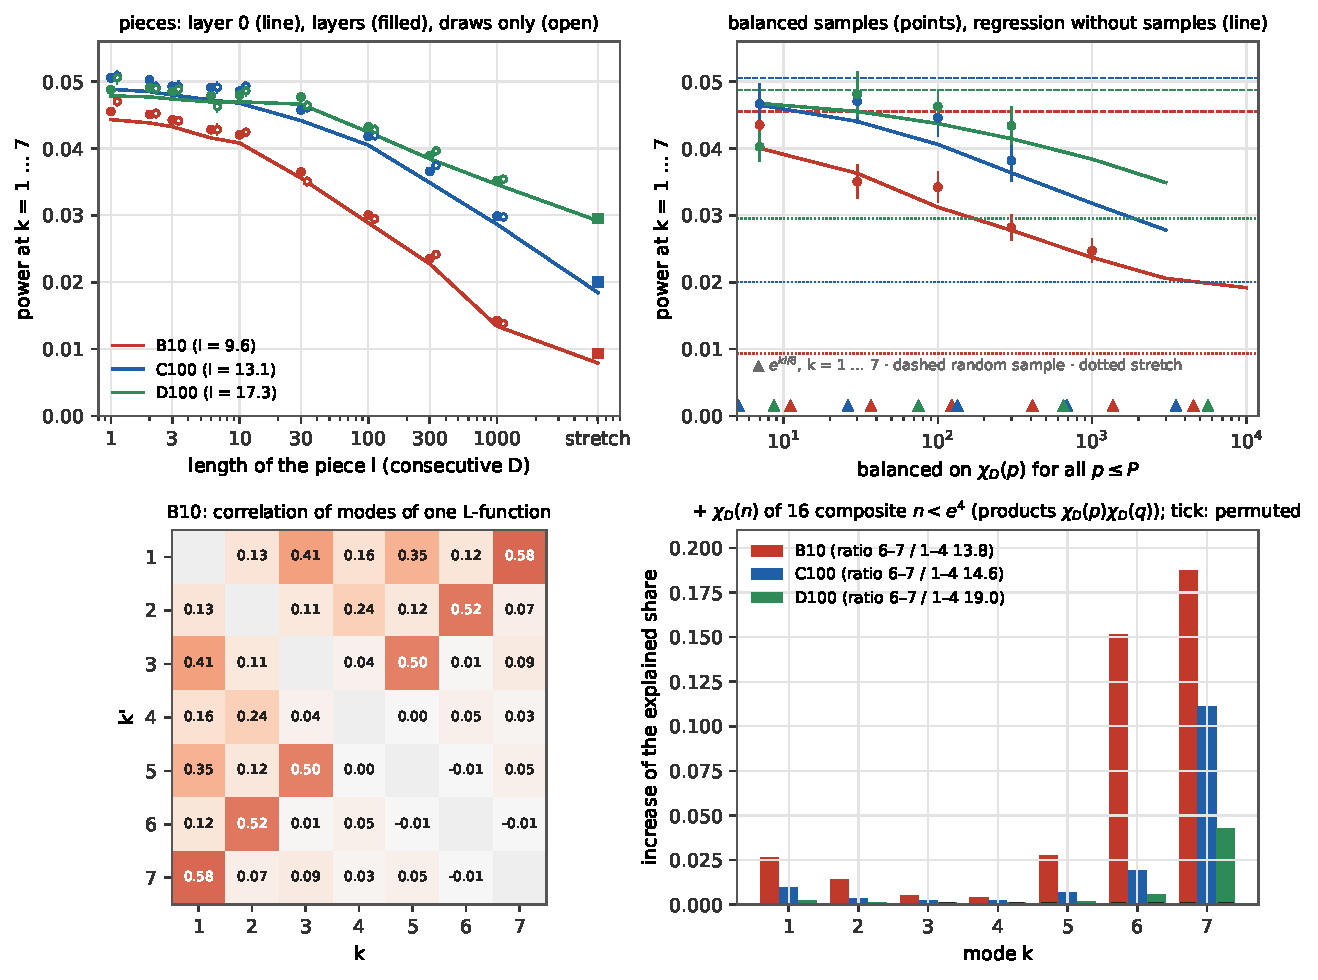
\includegraphics[width=0.95\textwidth,height=\textheight]{../figures/08_layers_en.pdf}
\caption{Figure 8. Upper left: low-frequency power of subsets of 6,074
L-functions from randomly placed pieces of \(\ell\) consecutive
discriminants (line layer 0 without draws, filled layered estimate ±1
error, open draws only, right one stretch). Upper right: samples
balanced on \(\chi_D(p)\) for \(p \le P\) (points ±1 error) and layer 0
from the regression (line); triangles \(e^{kl/8}\). Lower left:
correlation of the contributions of one L-function between the modes in
B10. Lower right: increase of the explained share of the variance of
every mode after adding \(\chi_D(n)\) of 16 composite \(n < e^4\), ticks
the null model.}
\end{figure}

\textbf{Pieces and triples.} The power falls with the length of the
piece. Already triples of consecutive discriminants lie below random
samples: 0.972 of the random value in B10 (4.7 standard errors) and
0.975 in C100 (4.3), as layer 0 predicts (0.976 and 0.983); in D100 the
decrease (0.995) is below the resolution, because at a larger conductor
the low modes are carried by larger primes, which three neighbours do
not balance.

\textbf{The offset of a few per cent.} The test statistic lies above
layer 0 by \(0.0012 \pm 0.0002 / 0.0017 \pm 0.0002 / 0.0009 \pm 0.0002\)
for random samples (2.7 / 3.5 / 1.9 \%), and the difference is positive
for all 30 designs; random noise would have both signs. It is a bias of
the estimate: a subset of 6,074 L-functions holds only 3.4 / 2.8 / 2.5
expected zeros in the lowest bin and about 20 in the second
(\(x < 0.1\)), where dividing by the square root of the observed count
is strongly non-linear. With the error from the expected count in these
two bins alone, 84 \% of the offset disappears in B10; with Pearson's
form everywhere the drawn statistic equals layer 0 within
\((1.5 \pm 1.5)\cdot10^{-6}\). A second-order delta expansion does not
capture it; three or four zeros are outside its range. The earlier
impression of about 5 \% was this offset together with the error of the
draws.

\textbf{Balanced samples.} A random sample can be held to the
composition of the whole family in \(\chi_D(p)\) and \(\chi_D(p)^2\) for
all primes \(p \le P\) (random start, then swaps that reduce the
imbalance weighted by \((\ln p)^2/p\); 100 samples per \(P\)). Its layer
0 follows from the regression of \(y_{ik}\) on these characters:
balancing keeps only the residual variance. In B10 the measured power is
\(0.0435 \pm 0.0029\), \(0.0350 \pm 0.0025\), \(0.0342 \pm 0.0024\),
\(0.0282 \pm 0.0019\), \(0.0247 \pm 0.0018\) for \(P\) = 7, 30, 100,
300, 1,000, and the linear statistic of the same samples agrees with the
regression in all 13 cases of the three families within three errors
(largest D100, \(P = 7\): 3.0). Mode \(k\) is balanced when \(P\)
reaches \(\ln p \approx k\,l/8\): in B10 (\(l = 9.6\)) mode 1 by the
primes up to 7, mode 4 up to 100 and mode 6 up to 1,000. With
\(P = 10^4\) layer 0 is 0.0192 in B10, still above the stretch (0.0079);
the rest is carried by larger primes and by composite \(n\).

\textbf{Coupling of modes and intermodulation.} The contributions of one
L-function to the modes \(k\) and \(8 - k\) are correlated: 1--7 / 2--6
/ 3--5 B10 0.58 / 0.52 / 0.50 · C100 0.47 / 0.42 / 0.40 · D100 0.39 /
0.35 / 0.35, whereas zeros as a Poisson process give exactly 0 (with
Pearson's form their covariance is \(N\) times the identity). Mode 8 is
the mean spacing of the zeros, and \(k\) and \(8 - k\) are its
sidebands. The coupling is of second order in the characters: adding to
the regression on all \(p \le 300\) the characters \(\chi_D(n)\) of the
16 squarefree composite \(n < e^4\) (products \(\chi_D(p)\chi_D(q)\) of
primes up to 23, for 30 and 42 of three) raises the explained share of
mode 7 by 0.188 / 0.111 / 0.043 and of mode 6 by 0.152 / 0.019 / 0.006,
of the modes 1--4 by at most 0.026; the same features permuted over the
L-functions give at most 0.0003. The small primes carry mode 1 (in B10
also 2), their products the mirror mode --- an intermodulation with the
carrier of the mean spacing. Balancing on \(\chi_D(n)\) of all
\(n \le 1{,}000\) lowers layer 0 to 0.0162 / 0.0253 / 0.0352, against
0.0237 / 0.0318 / 0.0384 with the primes alone; one stretch, which
balances all \(n\) below its width, has 0.0079 / 0.0185 / 0.0292.

\textbf{Filters in the frequency of the primes.} For one L-function and
an even test function \(\phi\) with compactly supported \(\hat\phi\),
the explicit formula has the prime \(p\) with the weight
\(\ln p/\sqrt p\) at the frequency \(u_p = \ln p/l\) (the term
\(\chi_D(p)\hat\phi(u_p)\)) and its square at \(2u_p\); in the cosine
modes this is \(k_p = 8u_p\). A subset fluctuates only through the means
\(\langle\chi_D(n)\rangle_{\mathcal S}\). For the whole family up to
\(X\) the average of \(\chi_D(p)\) over \(D\) is negligible for \(p\)
well below \(X\) (complete periods) and not for \(p \gtrsim X\); this is
the origin of the transition at \(|u| = 1\), in the Fourier transform of
the USp density and at the support condition \(|u| < 1\) of Rubinstein's
theorem {[}7{]} (under GRH, for the \(n\)-level densities
\(\sum|u_j| < 1\); extended to 2 by Gao {[}20{]} and Levinson--Miller
{[}21{]}; lower-order terms for extended support {[}17{]}). A stretch of
width \(\Delta\) near \(|D|\) has the same property only for
\(n \lesssim \Delta\): the mean runs over complete periods, and the
incomplete rest is bounded by the Pólya--Vinogradov inequality,
\(|\sum_{d \in I}(d/p)| < \sqrt p\ln p\) for every interval \(I\), so
for \(p\ln^2 p \ll \Delta\) the mean lies far below the
\(\Delta^{-1/2}\) of a random sample. (For fundamental discriminants the
squarefree condition breaks the exact periodicity; this is therefore a
heuristic, not a theorem.) The stretch is thus a low-pass filter in the
frequency of the primes up to \(u_c = \ln\Delta/l\) --- the analogue of
the support 1 with \(X\) replaced by \(\Delta\); for \(\Delta = |D|\),
\(u_c = 1\). In the modes \(k_c = 8u_c\) = 7.66 / 5.64 / 4.26 (B10 /
C100 / D100), and the ratio of layer 0 of one stretch to that of a
random sample is 0.10--0.28 / 0.20--0.43 / 0.34--0.44 below \(k_c\) and
--- / 0.44--0.54 / 0.61--0.93 above \(k_c\) (mean above / below 1.61 in
C100 and 1.97 in D100). The transition is gradual because the band
profile \(r_p\) rises smoothly with \(p/\Delta\) (Section 4.4).

A stratification by \(M\) is a comb filter. A fixed composition in
(sign, \(D \bmod 840\)) fixes the means of every function of these
residues: the lines of \(\chi_D(p)\) and \(\chi_D(p)^2\) for \(p\) = 2,
3, 5, 7 at \(k_p\) = 0.58, 0.91, 1.34, 1.62 in B10 (0.42--1.19 in C100,
0.32--0.90 in D100), the sign, and all products \(\chi_D(n)\),
\(n \mid 210\) --- the intermodulation lines. Layer 0 splits without
draws (regression on these features, finally all 840 occupied classes):
random sample → lines → + sign → + products → + products and lines times
sign → classes = B10 0.0443 → 0.0400 → 0.0400 → 0.0375 → 0.0374 →
0.0362; C100 0.0488 → 0.0465 → 0.0465 → 0.0456 → 0.0456 → 0.0450; D100
0.0479 → 0.0467 → 0.0467 → 0.0464 → 0.0464 → 0.0456 (the integer
allocation of the design gives 0.0369 / 0.0456 / 0.0469). The lines
carry 53 / 62 / 50 \% of the reduction, the products 33 / 24 / 17 \%,
the rest of the structure of the classes 14 / 14 / 33 \% and the sign
nothing. D mod 840 therefore acts in B10 (Section 4.4, \(z = -5.1\)) and
little at larger conductors, where the lines of 2, 3, 5, 7 lie below
mode 1.

\hypertarget{recomputation-by-layers-the-same-rules-another-principle}{%
\subsection{4.7 Recomputation by layers: the same rules, another
principle}\label{recomputation-by-layers-the-same-rules-another-principle}}

Sections 4.1--4.6 stand as they were computed. This section is an
extension: every number of Sections 4.3--4.5 that came from random
subsets is recomputed with the principle of Section 4.6 --- layer 0
without draws, draws only for the small difference of the actual test
--- and with the same rules: the same designs (random samples, the sign
and 19 moduli with the same largest-remainder allocation, \(m\) pieces
on the same grid of blocks), the same size of 6,074 L-functions and the
same statistic with the error from the observed count. For pieces the
exact layer 0 follows by conditioning on the two blocks of ranks \(r\)
and \(r + 1\) (the \(r\) longer pieces and the rest are then two
independent simple samples of blocks), with a total probability of 1
within \(10^{-12}\). Every design has 200 draws and more up to 1,800
until the error of the low-frequency power is below \(2\cdot10^{-4}\);
draw \(r\) of every design uses the same generator (common random
numbers). Fixed bands, one piece (\(m = 1\)) and one stretch over all
\(n - N + 1\) starting positions need no draws at all. The check of
layer 0 in the same draws (drawn Pearson statistic against layer 0)
gives for the 84 designs and four statistics a mean \(z^2\) of 1.13 and
\(|z| \le 3.0\). The error of the low-frequency power is 1.6--4.6 times
smaller than with the draws alone (median 3.7; smallest for 3 and 10
pieces in B10), that of the high modes and of \(\chi^2\) per bin 4--10
times.

{\small\begin{longtable}[]{@{}
  >{\raggedright\arraybackslash}p{(\columnwidth - 12\tabcolsep) * \real{0.1429}}
  >{\raggedright\arraybackslash}p{(\columnwidth - 12\tabcolsep) * \real{0.1429}}
  >{\raggedright\arraybackslash}p{(\columnwidth - 12\tabcolsep) * \real{0.1429}}
  >{\raggedright\arraybackslash}p{(\columnwidth - 12\tabcolsep) * \real{0.1429}}
  >{\raggedright\arraybackslash}p{(\columnwidth - 12\tabcolsep) * \real{0.1429}}
  >{\raggedright\arraybackslash}p{(\columnwidth - 12\tabcolsep) * \real{0.1429}}
  >{\raggedright\arraybackslash}p{(\columnwidth - 12\tabcolsep) * \real{0.1429}}@{}}
\toprule\noalign{}
\begin{minipage}[b]{\linewidth}\raggedright
stratification
\end{minipage} & \begin{minipage}[b]{\linewidth}\raggedright
B10 originally
\end{minipage} & \begin{minipage}[b]{\linewidth}\raggedright
B10 by layers
\end{minipage} & \begin{minipage}[b]{\linewidth}\raggedright
C100 originally
\end{minipage} & \begin{minipage}[b]{\linewidth}\raggedright
C100 by layers
\end{minipage} & \begin{minipage}[b]{\linewidth}\raggedright
D100 originally
\end{minipage} & \begin{minipage}[b]{\linewidth}\raggedright
D100 by layers
\end{minipage} \\
\midrule\noalign{}
\endhead
\bottomrule\noalign{}
\endlastfoot
random & 0.0440 & \(0.0456 \pm 0.0002\) & 0.0489 & \(0.0512 \pm 0.0003\)
& 0.0499 & \(0.0487 \pm 0.0002\) \\ \addlinespace[2pt]
sign only & 0.0452 (\(+0.6\)) & 0.0457 (\(+0.1\)) & 0.0490 (\(+0.0\)) &
0.0508 (\(-1.0\)) & 0.0497 (\(-0.0\)) & 0.0487 (\(-0.1\)) \\ \addlinespace[2pt]
\(D \bmod 3\) & 0.0468 (\(+1.5\)) & 0.0444 (\(-4.4\)) & 0.0508
(\(+0.9\)) & 0.0495 (\(-4.5\)) & 0.0480 (\(-0.6\)) & 0.0487
(\(-0.2\)) \\ \addlinespace[2pt]
\(D \bmod 5\) & 0.0479 (\(+1.0\)) & 0.0445 (\(-4.0\)) & 0.0510
(\(+0.6\)) & 0.0501 (\(-3.0\)) & 0.0573 (\(+1.3\)) & 0.0487
(\(-0.2\)) \\ \addlinespace[2pt]
\(D \bmod 7\) & 0.0436 (\(-0.2\)) & 0.0445 (\(-3.7\)) & 0.0508
(\(+0.9\)) & 0.0499 (\(-3.6\)) & 0.0487 (\(-0.3\)) & 0.0489
(\(+0.8\)) \\ \addlinespace[2pt]
\(D \bmod 8\) & 0.0414 (\(-1.5\)) & 0.0439 (\(-5.3\)) & 0.0480
(\(-0.5\)) & 0.0499 (\(-3.7\)) & 0.0457 (\(-1.4\)) & 0.0483
(\(-1.6\)) \\ \addlinespace[2pt]
\(D \bmod 9\) & 0.0424 (\(-0.5\)) & 0.0449 (\(-2.7\)) & 0.0493
(\(+0.1\)) & 0.0503 (\(-2.4\)) & 0.0552 (\(+0.9\)) & 0.0486
(\(-0.7\)) \\ \addlinespace[2pt]
\(D \bmod 13\) & 0.0442 (\(+0.1\)) & 0.0450 (\(-2.1\)) & 0.0485
(\(-0.1\)) & 0.0500 (\(-3.3\)) & 0.0512 (\(+0.2\)) & 0.0483
(\(-1.2\)) \\ \addlinespace[2pt]
\(D \bmod 16\) & 0.0425 (\(-0.9\)) & 0.0443 (\(-4.5\)) & 0.0518
(\(+1.4\)) & 0.0501 (\(-3.0\)) & 0.0478 (\(-0.6\)) & 0.0485
(\(-0.9\)) \\ \addlinespace[2pt]
\(D \bmod 24\) & 0.0431 (\(-0.3\)) & 0.0428 (\(-9.1\)) & 0.0503
(\(+0.4\)) & 0.0492 (\(-5.7\)) & 0.0425 (\(-1.4\)) & 0.0481
(\(-2.1\)) \\ \addlinespace[2pt]
\(D \bmod 40\) & 0.0390 (\(-1.7\)) & 0.0419 (\(-12.8\)) & 0.0464
(\(-0.7\)) & 0.0493 (\(-5.3\)) & 0.0422 (\(-1.4\)) & 0.0483
(\(-1.4\)) \\ \addlinespace[2pt]
\(D \bmod 41\) & 0.0445 (\(+0.3\)) & 0.0455 (\(-0.5\)) & 0.0505
(\(+0.8\)) & 0.0502 (\(-2.8\)) & 0.0438 (\(-2.0\)) & 0.0490
(\(+1.1\)) \\ \addlinespace[2pt]
\(D \bmod 120\) & 0.0420 (\(-0.7\)) & 0.0405 (\(-17.3\)) & 0.0506
(\(+0.5\)) & 0.0480 (\(-8.4\)) & 0.0555 (\(+0.9\)) & 0.0477
(\(-4.2\)) \\ \addlinespace[2pt]
\(D \bmod 130\) & 0.0460 (\(+0.6\)) & 0.0438 (\(-6.4\)) & 0.0531
(\(+1.4\)) & 0.0497 (\(-4.0\)) & 0.0508 (\(+0.2\)) & 0.0479
(\(-2.8\)) \\ \addlinespace[2pt]
\(D \bmod 131\) & 0.0451 (\(+0.6\)) & 0.0457 (\(+0.1\)) & 0.0505
(\(+0.7\)) & 0.0503 (\(-2.6\)) & 0.0547 (\(+1.2\)) & 0.0488
(\(+0.2\)) \\ \addlinespace[2pt]
\(D \bmod 260\) & 0.0447 (\(+0.2\)) & 0.0438 (\(-6.1\)) & 0.0526
(\(+1.0\)) & 0.0494 (\(-5.1\)) & 0.0485 (\(-0.2\)) & 0.0482
(\(-1.9\)) \\ \addlinespace[2pt]
\(D \bmod 360\) & 0.0402 (\(-2.1\)) & 0.0405 (\(-17.8\)) & 0.0468
(\(-1.1\)) & 0.0481 (\(-8.9\)) & 0.0456 (\(-1.3\)) & 0.0477
(\(-4.0\)) \\ \addlinespace[2pt]
\(D \bmod 369\) & 0.0434 (\(-0.2\)) & 0.0443 (\(-4.6\)) & 0.0551
(\(+1.7\)) & 0.0497 (\(-4.4\)) & 0.0511 (\(+0.3\)) & 0.0489
(\(+0.5\)) \\ \addlinespace[2pt]
\(D \bmod 520\) & 0.0425 (\(-0.8\)) & 0.0419 (\(-12.7\)) & 0.0476
(\(-0.7\)) & 0.0483 (\(-7.9\)) & 0.0479 (\(-0.6\)) & 0.0478
(\(-3.2\)) \\ \addlinespace[2pt]
\(D \bmod 800\) & 0.0415 (\(-0.8\)) & 0.0428 (\(-8.8\)) & 0.0479
(\(-0.3\)) & 0.0489 (\(-6.5\)) & 0.0395 (\(-2.4\)) & 0.0480
(\(-2.1\)) \\ \addlinespace[2pt]
\(D \bmod 840\) & 0.0359 (\(-5.1\)) & 0.0378 (\(-26.6\)) & 0.0462
(\(-1.4\)) & 0.0464 (\(-13.5\)) & 0.0518 (\(+0.6\)) & 0.0479
(\(-2.9\)) \\ \addlinespace[2pt]
consecutive bands & 0.0098 & 0.0098 (\(-7.5\)) & 0.0187 & 0.0187
(\(-23.0\)) & 0.0246 & 0.0246 (\(-7.1\)) \\ \addlinespace[2pt]
one stretch, all starts & --- & 0.0093 & --- & 0.0200 & --- & 0.0295 \\ \addlinespace[2pt]
\end{longtable}}

Section 4.4 by layers: power of the cosine coefficients
\(k = 1 \dots 7\) of subsets of 6,074 L-functions, originally (the table
of Section 4.4, 81--700 samples) and by layers (layer 0 exactly and
200--1,800 draws of the difference; error 0.0002--0.0003 for every
stratification), in brackets \(z\) against the random samples of the
same column. Consecutive bands and the stretch over all starting
positions are exact; the \(z\) of the bands uses the spread of the 9 /
100 / 10 bands.

\textbf{Residue classes.} With the precise values the stratifications
lower the low-frequency power in all three families. Layer 0, exact and
without error, is lower than for random samples for every modulus (by
0.00002--0.0074 in B10, 0.0001--0.0033 in C100 and 0.00005--0.0013 in
D100), and the layered estimates lie more than 3 errors below the random
samples for 15, 16 and 3 of the 19 moduli in B10, C100 and D100
(\(D \bmod 840\): \(z = -26.6\), \(-13.5\), \(-2.9\); \(D \bmod 120\)
and 360 in D100 \(-4.2\) and \(-4.0\)). The smallest effects belong to
the sign, 41 and 131, the stratifications with \(W_{100} \ge 0.96\)
(layer 0 lower by at most 0.0004); in C100 their \(z\) of \(-1.0\),
\(-2.8\) and \(-2.6\) is more than their exact difference of layer 0 (at
most 0.0003) explains and comes from the drawn part of the two columns,
so two moduli of C100 close to \(-3\) (\(D \bmod 5\) and 16, \(-3.02\)
and \(-3.04\)) are counted with this reservation. The sentence of
Section 4.4 that in C100 and D100 no stratification differs beyond
chance was the limit of the resolution of 30--700 samples. The size
keeps the conclusion of Section 4.4: \(D \bmod 840\) removes 17 / 9.5 /
1.6 \% of the random value, consecutive bands 79 / 64 / 50 \%, so the
balance of residue classes does not cause the low \(\chi^2\).

{\small\begin{longtable}[]{@{}
  >{\raggedright\arraybackslash}p{(\columnwidth - 16\tabcolsep) * \real{0.1111}}
  >{\raggedright\arraybackslash}p{(\columnwidth - 16\tabcolsep) * \real{0.1111}}
  >{\raggedright\arraybackslash}p{(\columnwidth - 16\tabcolsep) * \real{0.1111}}
  >{\raggedright\arraybackslash}p{(\columnwidth - 16\tabcolsep) * \real{0.1111}}
  >{\raggedright\arraybackslash}p{(\columnwidth - 16\tabcolsep) * \real{0.1111}}
  >{\raggedright\arraybackslash}p{(\columnwidth - 16\tabcolsep) * \real{0.1111}}
  >{\raggedright\arraybackslash}p{(\columnwidth - 16\tabcolsep) * \real{0.1111}}
  >{\raggedright\arraybackslash}p{(\columnwidth - 16\tabcolsep) * \real{0.1111}}
  >{\raggedright\arraybackslash}p{(\columnwidth - 16\tabcolsep) * \real{0.1111}}@{}}
\toprule\noalign{}
\begin{minipage}[b]{\linewidth}\raggedright
pieces \(m\)
\end{minipage} & \begin{minipage}[b]{\linewidth}\raggedright
B10 repetition
\end{minipage} & \begin{minipage}[b]{\linewidth}\raggedright
B10 by layers
\end{minipage} & \begin{minipage}[b]{\linewidth}\raggedright
B10 layer 0
\end{minipage} & \begin{minipage}[b]{\linewidth}\raggedright
C100 repetition
\end{minipage} & \begin{minipage}[b]{\linewidth}\raggedright
C100 by layers
\end{minipage} & \begin{minipage}[b]{\linewidth}\raggedright
C100 layer 0
\end{minipage} & \begin{minipage}[b]{\linewidth}\raggedright
D100 by layers
\end{minipage} & \begin{minipage}[b]{\linewidth}\raggedright
D100 layer 0
\end{minipage} \\
\midrule\noalign{}
\endhead
\bottomrule\noalign{}
\endlastfoot
1 & \(0.0095 \pm 0.0004\) & 0.0093\(^{*}\) & 0.0079 &
\(0.0206 \pm 0.0008\) & 0.0200\(^{*}\) & 0.0185 & 0.0295\(^{*}\) &
0.0292 \\ \addlinespace[2pt]
3 & \(0.0123 \pm 0.0005\) & \(0.0129 \pm 0.0002\) & 0.0117 &
\(0.0254 \pm 0.0009\) & \(0.0248 \pm 0.0002\) & 0.0232 &
\(0.0334 \pm 0.0002\) & 0.0324 \\ \addlinespace[2pt]
10 & \(0.0184 \pm 0.0007\) & \(0.0183 \pm 0.0002\) & 0.0176 &
\(0.0359 \pm 0.0012\) & \(0.0340 \pm 0.0002\) & 0.0322 &
\(0.0409 \pm 0.0002\) & 0.0401 \\ \addlinespace[2pt]
30 & \(0.0249 \pm 0.0009\) & \(0.0248 \pm 0.0002\) & 0.0238 &
\(0.0397 \pm 0.0013\) & \(0.0387 \pm 0.0002\) & 0.0371 &
\(0.0405 \pm 0.0002\) & 0.0397 \\ \addlinespace[2pt]
100 & \(0.0340 \pm 0.0011\) & \(0.0331 \pm 0.0002\) & 0.0321 &
\(0.0443 \pm 0.0016\) & \(0.0438 \pm 0.0002\) & 0.0420 &
\(0.0443 \pm 0.0002\) & 0.0433 \\ \addlinespace[2pt]
300 & \(0.0363 \pm 0.0013\) & \(0.0392 \pm 0.0002\) & 0.0377 &
\(0.0480 \pm 0.0015\) & \(0.0471 \pm 0.0002\) & 0.0452 &
\(0.0482 \pm 0.0002\) & 0.0475 \\ \addlinespace[2pt]
1000 & \(0.0439 \pm 0.0013\) & \(0.0428 \pm 0.0002\) & 0.0415 &
\(0.0483 \pm 0.0014\) & \(0.0489 \pm 0.0002\) & 0.0472 &
\(0.0507 \pm 0.0002\) & 0.0504 \\ \addlinespace[2pt]
2000 & \(0.0467 \pm 0.0016\) & \(0.0489 \pm 0.0002\) & 0.0473 &
\(0.0491 \pm 0.0014\) & \(0.0497 \pm 0.0002\) & 0.0480 &
\(0.0473 \pm 0.0002\) & 0.0454 \\ \addlinespace[2pt]
\end{longtable}}

Section 4.3 by layers: subsets of \(m\) pieces of consecutive
discriminants (random positions on a grid of blocks), originally
(repetition with 400 subsets, Section 4.3) and by layers, with the exact
layer 0. \(^{*}\) \(m = 1\): the mean over all \(n - N\) starting
positions, without draws.

\textbf{Pieces.} The values by layers agree with the repetition of
Section 4.3 within the joint error (largest B10 \(m = 300\): 2.3
errors), with an error 2.5--7 times smaller (6--7 times for
\(m \ge 100\)). Layer 0 splits exactly into the mean term (the square of
the mean contribution of the design) and the variance term. In B10 and
C100 the variance term grows monotonically with \(m\) towards the random
value, as the gradual loss of the effect requires; in D100, where the
subset is a tenth of the family, almost so (dips of 0.0004 at \(m = 30\)
and 0.0006 at \(m = 2{,}000\)). The points above the random value, B10
\(m = 2{,}000\) (\(0.0489 \pm 0.0002\) against \(0.0456 \pm 0.0002\))
and D100 \(m = 1{,}000\) (\(0.0507\) against \(0.0487\)), come from the
mean term --- \(0.0059\) against \(0.0002\) for random samples in B10,
\(0.0071\) against \(0.0029\) in D100 --- which is a property of the
design: with pieces of three on blocks of four the subset takes three of
every four consecutive discriminants, and the composition of the family
in this order is not that of a random sample.

\textbf{The line through two points.} With the original values the line
between random samples (\(W = 1\)) and consecutive bands gave
\(\chi^2 = 82.05\) for the 60 stratified subsets (\(p = 0.03\)). With
the precise values it gives \(\chi^2 = 841.8\) for 60 with the bands and
\(1{,}110.5\) with the stretch over all starts as the second point
(\(p < 10^{-130}\)), 42--43 of 60 deviations positive and a mean \(z\)
of \(+1.6\) / \(+1.8\). Without any draws, the reduction of layer 0 by
the stratifications is on average 0.89 / 0.56 / 0.39 of the reduction
the line gives in B10 / C100 / D100 (Figure 9, upper right). \(W_{100}\)
sets the direction, not the size, and the size falls with the conductor.
The same holds for the conductor dependence of the bands: the exact
ratio of the stretch over all starts to random samples is 0.204 / 0.391
/ 0.606 (originally \(0.22 \pm 0.11\), \(0.38 \pm 0.03\),
\(0.49 \pm 0.07\)) against \(W_k\) = 0.22 / 0.61 / 0.70 --- B10 agrees,
C100 and D100 lie below.

\textbf{The explicit formula and the dual term.} For one L-function the
explicit formula gives the count of zeros exactly; the part that depends
on the character has at the prime \(p\) the diagonal terms \(n = p^k\),
i.e.~the coefficient
\(-\frac{1}{\pi}\ln p \sum_{k\ \mathrm{odd}} p^{-k/2} I(k\ln p)\) on
\(\chi_D(p)\) and the even \(k\) on \(\chi_D(p)^2\), where \(I(w)\) is
the integral of \(\cos(wt)\) over the bin. Projected on the cosine modes
\(y_{ik}\) of Section 4.6 these weights can be compared, without a fit,
with the regression of \(y_{ik}\) on \(\chi_D(p)\) and \(\chi_D(p)^2\)
for \(p \le 100\) (175 coefficients per family). They describe the
direction but not the size: the slope is 0.52--0.60, and in windows of
\(x\) below 4 the fitted weight of \(\chi_D(2)\) is up to 51 errors from
the diagonal value (B10, \(x\) = 2.5--4). The missing part comes from
the term of the ratios conjecture that gives the sine of
\(W_{\mathrm{USp}}\) (the dual term). For the subfamily with
\(\chi_D(p) = e\) the local factor at \(p\) is
\((1 - e\,p^{-1/2-\gamma})/(1 - e\,p^{-1/2-\alpha})\) instead of the
family mean in both terms: the diagonal term gives back the weights
above, and the dual term changes by the factor \(A_e/A_p\) of the local
factors at \(\alpha = -it\), \(\gamma = it\). With these dual weights
added the slope is 0.995--0.999 in the three families and 0.94--1.01 by
mode (the largest deviation B10 \(k = 4\): \(0.978 \pm 0.004\)):

{\small\begin{longtable}[]{@{}
  >{\raggedright\arraybackslash}p{(\columnwidth - 14\tabcolsep) * \real{0.1250}}
  >{\raggedright\arraybackslash}p{(\columnwidth - 14\tabcolsep) * \real{0.1250}}
  >{\raggedright\arraybackslash}p{(\columnwidth - 14\tabcolsep) * \real{0.1250}}
  >{\raggedright\arraybackslash}p{(\columnwidth - 14\tabcolsep) * \real{0.1250}}
  >{\raggedright\arraybackslash}p{(\columnwidth - 14\tabcolsep) * \real{0.1250}}
  >{\raggedright\arraybackslash}p{(\columnwidth - 14\tabcolsep) * \real{0.1250}}
  >{\raggedright\arraybackslash}p{(\columnwidth - 14\tabcolsep) * \real{0.1250}}
  >{\raggedright\arraybackslash}p{(\columnwidth - 14\tabcolsep) * \real{0.1250}}@{}}
\toprule\noalign{}
\begin{minipage}[b]{\linewidth}\raggedright
family
\end{minipage} & \begin{minipage}[b]{\linewidth}\raggedright
slope, diagonal
\end{minipage} & \begin{minipage}[b]{\linewidth}\raggedright
slope, with dual term
\end{minipage} & \begin{minipage}[b]{\linewidth}\raggedright
windows \(\chi^2\) (30 coef.), diagonal → dual
\end{minipage} & \begin{minipage}[b]{\linewidth}\raggedright
explained share \(k = 1 \dots 4\), diagonal → dual
\end{minipage} & \begin{minipage}[b]{\linewidth}\raggedright
mod 8: exact / dual / diagonal
\end{minipage} & \begin{minipage}[b]{\linewidth}\raggedright
mod 840: exact / dual / diagonal
\end{minipage} & \begin{minipage}[b]{\linewidth}\raggedright
stretch: exact / dual / diagonal
\end{minipage} \\
\midrule\noalign{}
\endhead
\bottomrule\noalign{}
\endlastfoot
B10 & \(0.5227 \pm 0.0011\) & \(0.9948 \pm 0.0018\) & 6469 → 5.4 &
\(-0.53\) / \(-0.05\) / 0.33 / 0.55 → 0.56 / 0.69 / 0.76 / 0.80 &
0.00131 / 0.00130 / 0.00197 & 0.00737 / 0.00462 / 0.00995 & 0.0364 /
0.0325 / 0.0871 \\ \addlinespace[2pt]
C100 & \(0.5780 \pm 0.0004\) & \(0.9993 \pm 0.0007\) & 33797 → 9.2 &
\(-0.32\) / 0.12 / 0.40 / 0.52 → 0.55 / 0.71 / 0.78 / 0.76 & 0.00074 /
0.00074 / 0.00121 & 0.00328 / 0.00178 / 0.00358 & 0.0304 / 0.0230 /
0.0651 \\ \addlinespace[2pt]
D100 & \(0.5980 \pm 0.0019\) & \(0.9993 \pm 0.0029\) & 1746 → 27.8 &
0.08 / 0.36 / 0.47 / \(-0.07\) → 0.54 / 0.68 / 0.68 / 0.10 & 0.00032 /
0.00033 / 0.00060 & 0.00095 / 0.00099 / 0.00224 & 0.0187 / 0.0122 /
0.0336 \\ \addlinespace[2pt]
\end{longtable}}

Weights of the explicit formula against the regression of the
contributions \(y_{ik}\) of single L-functions on \(\chi_D(p)\),
\(p \le 100\): slope of the fitted against the predicted weights (all 7
modes), \(\chi^2\) of fitted minus predicted in 5 windows of \(x\) for
\(p\) = 2 \ldots{} 13, share of the variance of \(y_{ik}\) explained by
the prediction from all \(p \le 1{,}000\) without a fit, and the
reduction of layer 0 by \(D \bmod 8\), \(D \bmod 840\) and one stretch
predicted from the characters alone (prime by prime) against the exact
value from the zeros.

With the dual term \(\chi^2\) per coefficient is 0.45 / 0.31 / 0.78 for
\(\chi_D(p)\) (175 coefficients each), against 1,497 / 7,787 / 361 with
the diagonal terms alone. The prediction from the characters alone,
without zeros, then gives the stratification by \(D \bmod 8\), which
fixes only \(\chi_D(2)\), within 3 \%; for \(D \bmod 840\) it gives 63 /
54 / 104 \% of the exact reduction and for the stretch 89 / 76 / 65 \%.
A prediction prime by prime does not contain the products
\(\chi_D(p)\chi_D(q)\) that carry the coupling of modes in Section 4.6;
they are the natural candidate for the rest in B10 and C100, which is
not computed here. The modes 5--7 of C100 and D100 are carried by primes
above 1,000 (\(\ln p \approx k\,l/8\)) and are explained only to 4--18
\% by \(p \le 1{,}000\).

{\small\begin{longtable}[]{@{}
  >{\raggedright\arraybackslash}p{(\columnwidth - 8\tabcolsep) * \real{0.2000}}
  >{\raggedright\arraybackslash}p{(\columnwidth - 8\tabcolsep) * \real{0.2000}}
  >{\raggedright\arraybackslash}p{(\columnwidth - 8\tabcolsep) * \real{0.2000}}
  >{\raggedright\arraybackslash}p{(\columnwidth - 8\tabcolsep) * \real{0.2000}}
  >{\raggedright\arraybackslash}p{(\columnwidth - 8\tabcolsep) * \real{0.2000}}@{}}
\toprule\noalign{}
\begin{minipage}[b]{\linewidth}\raggedright
family
\end{minipage} & \begin{minipage}[b]{\linewidth}\raggedright
sign
\end{minipage} & \begin{minipage}[b]{\linewidth}\raggedright
\(N_{\mathrm{eff}}(a)\), \(a\) = 0.3 \ldots{} 0.7
\end{minipage} & \begin{minipage}[b]{\linewidth}\raggedright
mean \(x_1\) \(-\) USp, \(a\) = 0.3 / 0.5 / 0.7 (error)
\end{minipage} & \begin{minipage}[b]{\linewidth}\raggedright
KS / critical, \(a\) = 0.3 / 0.5 / 0.7
\end{minipage} \\
\midrule\noalign{}
\endhead
\bottomrule\noalign{}
\endlastfoot
B10 & even & 1.64 \ldots{} 2.05 & \(+0.0285\) / \(+0.0102\) /
\(-0.0041\) (0.0015) & 6.28 / 3.09 / 2.16 \\ \addlinespace[2pt]
B10 & odd & 2.33 \ldots{} 2.37 & \(+0.0000\) / \(+0.0002\) / \(-0.0023\)
(0.0015) & 0.34 / 0.37 / 0.66 \\ \addlinespace[2pt]
R10 & even & 2.51 \ldots{} 2.81 & \(+0.0134\) / \(+0.0073\) /
\(+0.0005\) (0.0016) & 2.94 / 1.87 / 1.00 \\ \addlinespace[2pt]
R10 & odd & 3.24 \ldots{} 3.26 & \(-0.0011\) / \(-0.0010\) / \(-0.0019\)
(0.0016) & 0.35 / 0.34 / 0.43 \\ \addlinespace[2pt]
C100 & even & 2.28 \ldots{} 2.61 & \(+0.0153\) / \(+0.0072\) /
\(-0.0012\) (0.0005) & 10.52 / 6.18 / 3.54 \\ \addlinespace[2pt]
C100 & odd & 3.00 \ldots{} 3.04 & \(-0.0005\) / \(-0.0005\) /
\(-0.0017\) (0.0005) & 0.44 / 0.43 / 0.99 \\ \addlinespace[2pt]
D100 & even & 3.14 \ldots{} 3.36 & \(+0.0067\) / \(+0.0038\) /
\(+0.0000\) (0.0016) & 1.51 / 1.10 / 0.62 \\ \addlinespace[2pt]
D100 & odd & 3.87 \ldots{} 3.88 & \(-0.0004\) / \(-0.0002\) /
\(-0.0005\) (0.0016) & 0.41 / 0.39 / 0.42 \\ \addlinespace[2pt]
E10 & even & 4.11 \ldots{} 4.24 & \(+0.0023\) / \(+0.0013\) /
\(-0.0002\) (0.0037) & 0.44 / 0.39 / 0.35 \\ \addlinespace[2pt]
E10 & odd & 4.84 \ldots{} 4.82 & \(-0.0019\) / \(-0.0017\) / \(-0.0016\)
(0.0037) & 0.47 / 0.45 / 0.45 \\ \addlinespace[2pt]
\end{longtable}}

First zero with \(N_{\mathrm{eff}}\) calibrated on \([0, a]\): mean
\(x_1\) of the data minus USp\((2N_{\mathrm{eff}}(a))\) and KS distance
divided by the critical value (5 \%).

\textbf{The first zero: calibration and the two-level part.} For the
count \(N(a)\) of zeros in \([0, a]\),
\(P(x_1 \le a) = E[N(a)] - \sum_{k \ge 2} P(N(a) \ge k)\); the first
term is fixed by the one-level density, the rest needs the two-level
density. In USp\((2N)\) the zeros in \([0, a]\) form a determinantal
process with the kernel \(S_N(x - y) - S_N(x + y)\), so \(N(a)\) is a
sum of independent Bernoulli variables with the eigenvalues of the
kernel. Up to \(a = \frac12\) the second factorial moment
\(E[N(N - 1)]\), the integral of the two-level density over
\([0, a]^2\), is at most 0.0004 in the model and 0.00013 in the data,
and the two-level part \(\sum_{k \ge 2} P(N \ge k)\) at most 0.0002 and
0.00007, so \(F(\frac12)\) is the one-level density and the calibration
of \(N_{\mathrm{eff}}\) on \([0, \frac12]\) fixes it; at \(a = 1\) it
matters (C100, even characters: \(E[N(1)] - F(1)\) lies 0.028 below the
model and \(F(1)\) 0.014). With \(N_{\mathrm{eff}}\) fixed on \([0, a]\)
for \(a\) = 0.3 \ldots{} 0.7 separately for each sign, the shift of the
mean first zero of even characters of Section 4.5 shrinks with \(a\) and
at \(a = 0.7\) is at most 0.0041 in absolute value in all five families
(C100 \(+0.0153 \to -0.0012 \pm 0.0005\); it changes sign between 0.6
and 0.7 in B10, C100 and E10), while for odd characters
\(N_{\mathrm{eff}}\) hardly depends on \(a\) (3.00--3.04 in C100) and
the mean agrees within 0.0023 at every calibration (Figure 9, lower
right). The shift of the mean is therefore not a property of the zeros:
the density of the ratios conjecture for even characters is not
\(W_{\mathrm{USp}(2N)}\) for any single \(N\). The deviation of the
shape remains: in B10 and C100 the KS distance of even characters stays
above the critical value at every calibration (2.2--10.5 times), in D100
it falls below from \(a = 0.6\) and in R10 at \(a = 0.7\) (0.996 of the
critical value), in E10 (6,000 L) it is below everywhere; odd characters
are below everywhere.

\textbf{Completeness of the zeros.} The zeros were found by
\texttt{lfunzeros} of PARI/GP, which looks for sign changes of the Hardy
function with a step of the mean spacing divided by 8; two zeros closer
than one step give no sign change and are both missed. For random
samples of 3,000 L-functions of B10 and C100 the step / 8 reproduces the
data in every L-function (within \(10^{-6}\)), and the step / 64 finds
additional zeros in one L-function of B10 (\(D = -78{,}671\): two zeros
at \(x\) = 3.307 and 3.330, \(t\) = 2.169 and 2.183) and in none of
C100. Above \(x = 2\) this is a relative deficit of the density of order
\(10^{-4}\), far below the statistical error of a bin (0.6 \% in C100).
The generator \texttt{ks\_nuly.py} now has the option \texttt{-\/-divz}
(default 32, about 25 \% slower); the published blocks keep the step / 8
and their checksums.

\begin{figure}
\centering
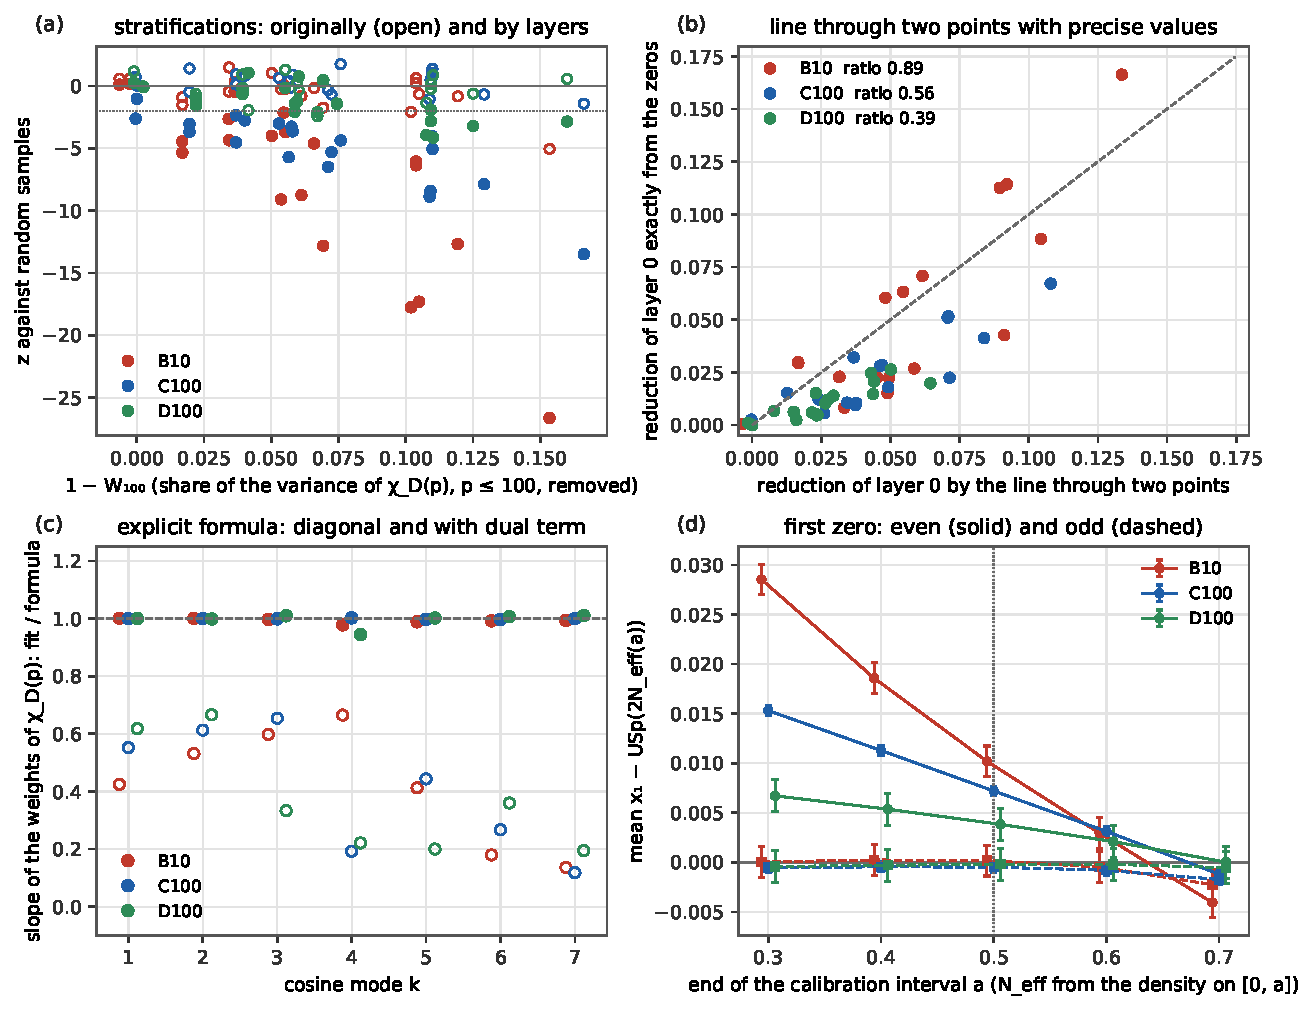
\includegraphics[width=0.95\textwidth,height=\textheight]{../figures/09_recomputation_en.pdf}
\caption{Figure 9. Recomputation by layers. (a) \(z\) of the 20
stratifications against random samples, originally (Section 4.4, open)
and by layers (filled), against the share \(1 - W_{100}\) of the
variance of \(\chi_D(p)\), \(p \le 100\), that the stratification
removes. (b) Reduction of layer 0 by the stratifications, exactly from
the zeros, against the line through two points; dashed equality, in the
legend the mean ratio. (c) Slope of the fitted weights of \(\chi_D(p)\)
against the explicit formula by cosine mode, diagonal terms alone (open)
and with the dual term of the ratios conjecture (filled). (d) Mean first
zero minus USp\((2N_{\mathrm{eff}}(a))\) with \(N_{\mathrm{eff}}\) fixed
by the density of the ratios conjecture on \([0, a]\), even (solid) and
odd (dashed) characters; dotted \(a = \frac12\), the calibration of
Section 4.5.}
\end{figure}

\hypertarget{enlargement-at-d-1010-the-family-e100}{%
\subsection{\texorpdfstring{4.8 Enlargement at \(|D| = 10^{10}\): the
family
E100}{4.8 Enlargement at \textbar D\textbar{} = 10\^{}\{10\}: the family E100}}\label{enlargement-at-d-1010-the-family-e100}}

At the largest conductor the errors were set by the number of
L-functions, not of zeros: E10 has 12,153. The family was therefore
continued without overlap up to \(|D| = 10^{10} + 2\cdot10^5\): 109,404
further L-functions in 900 blocks with 471,278 zeros, computed on the
second computer with the same revision of the generator (SHA-256
\texttt{e4a8325f…}, PARI/GP 2.17.2, step of the search mean spacing / 8
as for all other families) in 14 hours on nine processes; every block
agrees with its checksum. Together with E10 they form the family E100 of
this section: all 121,557 fundamental discriminants with
\(10^{10} < |D| < 10^{10} + 2\cdot10^5\) (60,772 even, 60,785 odd), ten
times E10 at the same \(l = 21.88\). The scripts of Sections 4.1--4.7
were run on E100 unchanged (option \texttt{-\/-families\ E100}); the
earlier sections and their numbers stay as they are.

The family E10 and the family E100 at \(|D| = 10^{10}\): \(\chi^2\) per
bin of 0.05 of the one-level density against the models (all / even /
odd for the ratios conjecture), density in \([0, \frac12]\), mean first
zero minus USp\((2N_{\mathrm{eff}})\) (\(N_{\mathrm{eff}}\) on
\([0, \frac12]\)) and KS distance divided by the critical value (5 \%).

{\small\begin{longtable}[]{@{}
  >{\raggedright\arraybackslash}p{(\columnwidth - 4\tabcolsep) * \real{0.3333}}
  >{\raggedright\arraybackslash}p{(\columnwidth - 4\tabcolsep) * \real{0.3333}}
  >{\raggedright\arraybackslash}p{(\columnwidth - 4\tabcolsep) * \real{0.3333}}@{}}
\toprule\noalign{}
\begin{minipage}[b]{\linewidth}\raggedright
\end{minipage} & \begin{minipage}[b]{\linewidth}\raggedright
E10
\end{minipage} & \begin{minipage}[b]{\linewidth}\raggedright
E100
\end{minipage} \\
\midrule\noalign{}
\endhead
\bottomrule\noalign{}
\endlastfoot
L-functions (even / odd) & 12,153 (6,084 / 6,069) & 121,557 (60,772 /
60,785) \\ \addlinespace[2pt]
\(\chi^2\), ratios conjecture & 0.661 / 0.813 / 0.835 & 0.759 / 0.785 /
0.821 \\ \addlinespace[2pt]
\(\chi^2\), without \(A\) and \(\Delta\) & 2.57 & 16.48 \\ \addlinespace[2pt]
\(\chi^2\), USp\((2N)\), \(N = l/2\) & 3.42 & 24.44 \\ \addlinespace[2pt]
\(\chi^2\), USp & 7.81 & 66.75 \\ \addlinespace[2pt]
density in \([0, \frac12]\) (ratios conjecture 0.5267, USp 0.4105) &
\(0.5273 \pm 0.0093\) & \(0.5291 \pm 0.0030\) \\ \addlinespace[2pt]
\(x_1 - {}\)USp\((2N_{\mathrm{eff}})\), even & \(+0.0013 \pm 0.0037\) &
\(+0.0016 \pm 0.0012\) \\ \addlinespace[2pt]
\(x_1 - {}\)USp\((2N_{\mathrm{eff}})\), odd & \(-0.0017 \pm 0.0037\) &
\(-0.0009 \pm 0.0012\) \\ \addlinespace[2pt]
KS / critical value, even / odd & 0.34 / 0.37 & 0.73 / 0.46 \\ \addlinespace[2pt]
\end{longtable}}

\textbf{One-level density.} With ten times the data the density still
follows the ratios conjecture: \(\chi^2\) per bin 0.759, while without
the arithmetic factor \(A\) and the term with \(\Delta\) it is 16.5,
against USp\((2N)\) with \(N = l/2\) 24.4 and against the Katz--Sarnak
limit 66.7 (E10: 2.6, 3.4 and 7.8). The density in \([0, \frac12]\) is
\(0.5291 \pm 0.0030\) against 0.5267 for the ratios conjecture and
0.4105 for USp, 39 errors above the limit at \(|D| = 10^{10}\). As a
consecutive family E100 has \(\chi^2\) below 0.95, as Section 4.3 leads
one to expect.

Consecutive stretches, stratifications and the explicit formula over the
conductor, by layers (Section 4.7): ratio of one stretch of 6,074
consecutive discriminants over all starting positions to random samples
(exact), reduction by \(D \bmod 840\) with \(z\), number of the 19
moduli more than 3 errors below random samples, exact reduction of layer
0 by the stratifications relative to the line through two points, share
of the exact reduction of one stretch predicted from the characters
alone (prime by prime, with the dual term), and slope of the weights of
\(\chi_D(p)\) with the dual term (diagonal terms alone in brackets).

{\small\begin{longtable}[]{@{}
  >{\raggedright\arraybackslash}p{(\columnwidth - 14\tabcolsep) * \real{0.1250}}
  >{\raggedright\arraybackslash}p{(\columnwidth - 14\tabcolsep) * \real{0.1250}}
  >{\raggedright\arraybackslash}p{(\columnwidth - 14\tabcolsep) * \real{0.1250}}
  >{\raggedright\arraybackslash}p{(\columnwidth - 14\tabcolsep) * \real{0.1250}}
  >{\raggedright\arraybackslash}p{(\columnwidth - 14\tabcolsep) * \real{0.1250}}
  >{\raggedright\arraybackslash}p{(\columnwidth - 14\tabcolsep) * \real{0.1250}}
  >{\raggedright\arraybackslash}p{(\columnwidth - 14\tabcolsep) * \real{0.1250}}
  >{\raggedright\arraybackslash}p{(\columnwidth - 14\tabcolsep) * \real{0.1250}}@{}}
\toprule\noalign{}
\begin{minipage}[b]{\linewidth}\raggedright
family
\end{minipage} & \begin{minipage}[b]{\linewidth}\raggedright
\(l\)
\end{minipage} & \begin{minipage}[b]{\linewidth}\raggedright
stretch / random
\end{minipage} & \begin{minipage}[b]{\linewidth}\raggedright
\(D \bmod 840\)
\end{minipage} & \begin{minipage}[b]{\linewidth}\raggedright
moduli below \(-3\)
\end{minipage} & \begin{minipage}[b]{\linewidth}\raggedright
strata / line
\end{minipage} & \begin{minipage}[b]{\linewidth}\raggedright
from the characters
\end{minipage} & \begin{minipage}[b]{\linewidth}\raggedright
slope of the weights
\end{minipage} \\
\midrule\noalign{}
\endhead
\bottomrule\noalign{}
\endlastfoot
B10 & 9.62 & 0.204 & 17.2 \% (\(-26.6\)) & 15 & 0.89 & 89 \% & 0.995
(0.523) \\ \addlinespace[2pt]
C100 & 13.06 & 0.391 & 9.5 \% (\(-13.5\)) & 16 & 0.56 & 76 \% & 0.999
(0.578) \\ \addlinespace[2pt]
D100 & 17.28 & 0.606 & 1.6 \% (\(-2.9\)) & 3 & 0.39 & 65 \% & 0.999
(0.598) \\ \addlinespace[2pt]
E100 & 21.88 & 0.622 & 2.2 \% (\(-4.0\)) & 2 & 0.20 & 42 \% & 1.001
(0.608) \\ \addlinespace[2pt]
\end{longtable}}

\textbf{Consecutive stretches and residue classes.} One stretch of 6,074
consecutive discriminants keeps over all 115,484 starting positions
0.622 of the low-frequency power of random samples (exact, without
draws): the effect of consecutive families persists at \(10^{10}\), and
between \(10^8\) and \(10^{10}\) it hardly decreases (0.606 → 0.622),
although over a stretch the means of \(\chi_D(p)\), \(p \le 100\), keep
only 4.3 \% of their random variance (\(W_{100}\)). The stratifications
behave as in D100: \(D \bmod 840\) lowers the power by 2.2 \%
(\(z = -4.0\)), two of 19 moduli lie more than 3 errors below; the line
through two points fails (\(\chi^2 = 218\) for 20), and the exact
reduction is 0.20 of the line, continuing 0.89 / 0.56 / 0.39. The
explicit formula with the dual term describes E100 as the other families
(slope \(1.0007 \pm 0.0027\), \(\chi^2\) per coefficient 0.92; diagonal
terms alone 0.608), but the part of the reduction of one stretch that
the characters give prime by prime falls with the conductor, 89 / 76 /
65 / 42 \%; the rest, which a prediction prime by prime does not contain
(products \(\chi_D(p)\chi_D(q)\), Section 4.6), grows with \(l\).

\textbf{The first zero.} Odd characters agree with
USp\((2N_{\mathrm{eff}})\) also at the threefold smaller error
(\(-0.0009 \pm 0.0012\), KS 0.46 of the critical value). For even
characters the shift of the mean (\(N_{\mathrm{eff}}\) on
\([0, \frac12]\), Section 4.5) is \(+0.0016 \pm 0.0012\), 2.3 errors
below the value 0.0043 of the law \(0.094/l\) fitted in Section 4.5 to
B10, C100, R10, D100 and E10, where E10 had an error of 0.0037. With
E100 in place of E10 \(c/l\) is still acceptable (\(p = 0.17\)), but a
free power \(c\,l^{-a}\) gives \(a = 1.60\) (1.27--1.95) instead of 1.33
(0.91--1.74), and the data do not decide between \(1/l\) and \(1/l^2\).
The deviation of the shape is clearer. At \(x_1 = 1\) the difference
\(F(1) - \mathrm{USp}(2N_{\mathrm{eff}})\) of even characters is
\(-0.0029 \pm 0.0015\) in E100, against \(-0.0069\) from the power law
fitted to B10, C100, R10 and D100 (\(a = 1.34\); 2.7 errors), and one
power law no longer fits all five families (\(p = 0.09\); \(1/l\):
\(p = 0.003\), \(1/l^2\): \(p = 0.04\)). With \(N_{\mathrm{eff}}\)
calibrated on \([0, a]\) the KS distance of even characters stays below
the critical value at every calibration (0.56--0.89 of it), and the
shift of the mean goes from \(+0.0026\) (\(a = 0.3\)) to \(+0.0000\)
(\(a = 0.7\)) (Figure 10, lower right). At \(10^{10}\) the
even-character term is thus at the limit of the resolution of 60,000
L-functions (1.3 and 1.9 errors), and over the conductor it falls faster
than \(1/l\) between \(l = 17\) and \(22\). Whether this is a
finite-size effect of the comparison with a single
USp\((2N_{\mathrm{eff}})\) or a property of the family needs the first
zero from the ratios conjecture (open).

The enlargement confirms Sections 4.1--4.7 at \(10^{10}\) with errors
about three times smaller and changes one statement: the law \(0.094/l\)
of the even-character shift (Section 4.5) is no longer preferred, and
the deviation of the shape falls faster than \(1/l\).

\begin{figure}
\centering
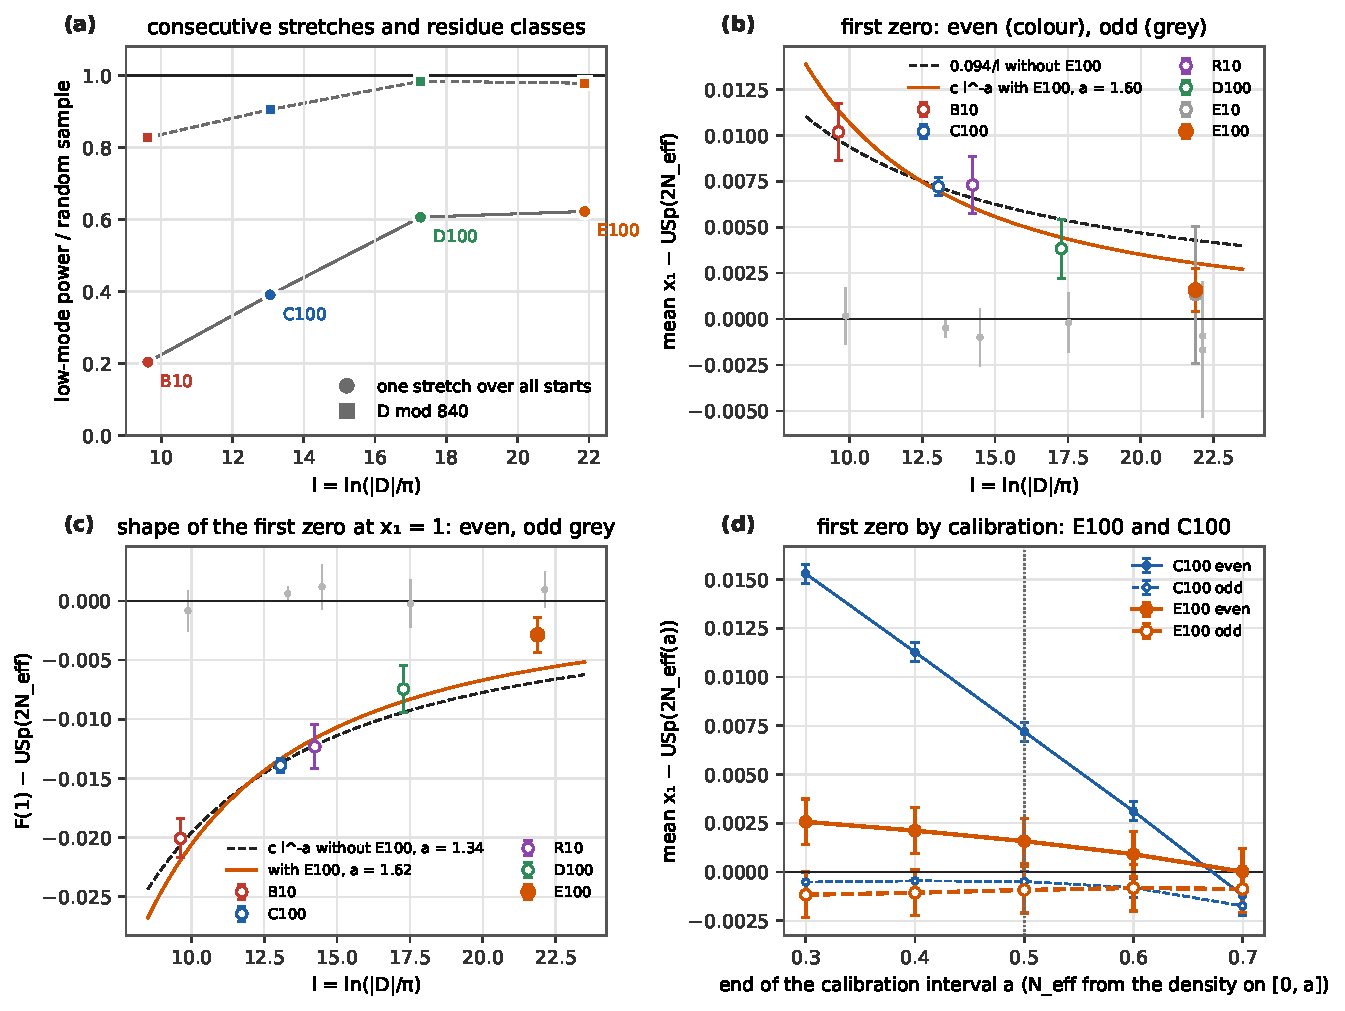
\includegraphics[width=0.95\textwidth,height=\textheight]{../figures/10_e100_en.pdf}
\caption{Figure 10. Enlargement at \(|D| = 10^{10}\) (family E100,
121,557 L-functions). (a) Low-frequency power of one consecutive stretch
over all starting positions (circles) and of samples stratified by
\(D \bmod 840\) (squares) relative to random samples, by layers. (b)
Shift of the mean first zero of even characters against
USp\((2N_{\mathrm{eff}})\) (\(N_{\mathrm{eff}}\) on \([0, \frac12]\))
over \(l = \ln(|D|/\pi)\); open the families of Section 4.5, filled
E100; dashed the law \(0.094/l\) without E100, solid \(c\,l^{-a}\) with
E100; odd characters grey. (c) Deviation of the shape,
\(F(1) - \mathrm{USp}(2N_{\mathrm{eff}})\) at \(x_1 = 1\), for even
characters with \(c\,l^{-a}\) fitted without (dashed) and with E100
(solid); odd grey. (d) Mean first zero minus
USp\((2N_{\mathrm{eff}}(a))\) with \(N_{\mathrm{eff}}\) calibrated on
\([0, a]\), E100 (thick) and C100 (thin), even (filled) and odd (open).}
\end{figure}

\hypertarget{statements-and-their-status}{%
\section{5. Statements and their
status}\label{statements-and-their-status}}

{\small\begin{longtable}[]{@{}
  >{\raggedright\arraybackslash}p{(\columnwidth - 2\tabcolsep) * \real{0.5435}}
  >{\raggedright\arraybackslash}p{(\columnwidth - 2\tabcolsep) * \real{0.4565}}@{}}
\toprule\noalign{}
\begin{minipage}[b]{\linewidth}\raggedright
statement
\end{minipage} & \begin{minipage}[b]{\linewidth}\raggedright
status
\end{minipage} \\
\midrule\noalign{}
\endhead
\bottomrule\noalign{}
\endlastfoot
The one-level density of the low zeros of quadratic Dirichlet
L-functions at finite conductor is given by the ratios conjecture
(Conrey--Snaith form, adapted to all fundamental discriminants). & Known
theory {[}8, 9{]}, conjectural; consistent here with 795,381 L-functions
in eleven families up to \(|D| = 10^{10}\), \(\chi^2\) per bin
0.54--1.19, density near the central point within 1.2 errors in 33
combinations; at \(|D| = 10^{10}\) also with the 121,557 L-functions of
E100 (\(\chi^2\) 0.759, Section 4.8). \\ \addlinespace[2pt]
The Katz--Sarnak limit USp is not reached at these conductors. & Known
{[}7, 9{]}; measured here: at \(|D| = 10^{10}\) the density in
\([0, \frac12]\) is 12.6 errors above USp and follows the ratios
conjecture for one discriminant; in E100 39 errors (Section 4.8). \\ \addlinespace[2pt]
Families of consecutive discriminants have smaller fluctuations of the
density at low frequencies \(u < \ln\Delta/\ln(|D|/\pi)\) than random
samples, because the averages of \(\chi_D(p)\) for \(p\) below the
length \(\Delta\) of the stretch run over nearly complete periods. &
Measured here (0.23 / 0.36 / 0.48 of the low-frequency power at
\(|D| \approx 5\cdot10^4\) / \(1.5\cdot10^6\) / \(10^8\); 5.9 / 10.2 /
4.3 errors); the mechanism is the periodicity used in mean-value
theorems {[}14, 15{]}, and \(u_c\) is the analogue for a short family of
the transition at support 1 {[}7, 16, 17{]}; tested by subsets of \(m\)
pieces. As far as we have been able to find, the size of the effect for
consecutive subfamilies has not been quantified before. \\ \addlinespace[2pt]
The low \(\chi^2\) of the family \(10^4 < |D| \le 2\cdot10^4\) is
exceptional. & Rejected here: it is the lowest of nine consecutive
bands, 1.5 standard deviations below their mean. \\ \addlinespace[2pt]
The low \(\chi^2\) is caused by the balance of residue classes of \(D\)
modulo the smallest primes. & Rejected here for 19 moduli (3 to 840 and
131) and the sign, with an independent repetition: in C100 and D100 no
stratification beyond chance, in B10 only \(D \bmod 840\)
(\(z = -5.1\)); balancing \(D \bmod 8\) (\(\chi_D(2)\)) or the sign is
not decisive. Section 4.7, by layers: every modulus lowers the exact
layer 0 slightly, by more than 3 errors for 15 / 16 / 3 of the 19 moduli
in B10 / C100 / D100; \(D \bmod 840\) removes 17 / 9.5 / 1.6 \% of the
random value against 79 / 64 / 50 \% for the bands, so the rejection
stands. \\ \addlinespace[2pt]
A stratification by \(D \bmod M\) fixes the means of \(\chi_D(p)\) only
for the primes dividing \(M\) (for \(p = 2\) only when \(8 \mid M\)). &
Consistent here (elementary periodicity): the exact variance of
stratified sampling is at most 0.07 of the random variance for
\(p \mid M\) and 1.000--1.014 for the other primes; random samples agree
with sampling from a finite population within 0.4 \%. \\ \addlinespace[2pt]
The low-frequency power of the zeros of a subset follows the remaining
variance \(W\) of the sums of \(\chi_D(p)\) over small primes. &
Measured here: in direction for all 60 stratified subsets; in size only
at the edge --- \(\chi^2 = 82.05\) for 60 with the joint errors
(\(p = 0.03\)), 42 of 60 deviations positive. As far as we have been
able to find, not described before. Section 4.7: with the values by
layers rejected in size (\(\chi^2 = 841.8\) for 60, \(p < 10^{-130}\));
exactly, the stratifications give 0.89 / 0.56 / 0.39 of the reduction of
the line. \\ \addlinespace[2pt]
Equal weights \((\ln p)^2/p\) for all primes of the low modes predict
the size. & Rejected here: the shift of the deviations disappears, but
\(\chi^2 = 91.0\) for 60 (\(p = 0.006\)) and B10 mod 840 lies 4.1 errors
below. \\ \addlinespace[2pt]
The \(k\)-weighted share \(W_k\) of the band profile predicts the size
of the conductor dependence of consecutive bands. & Rejected here: the
order is right (\(W_k\) \(0.22 \to 0.61 \to 0.70\), measured ratio
\(0.22 \to 0.38 \to 0.49\)), the size for C100 is off by 7 errors; open.
Section 4.7: exact ratio 0.204 / 0.391 / 0.606. \\ \addlinespace[2pt]
USp\((2N)\) with \(N = \frac12\ln(|D|/\pi)\) describes the first zero. &
Rejected here (KS 1.6 to 53 times the critical value). \\ \addlinespace[2pt]
USp\((2N_{\mathrm{eff}})\) with \(N_{\mathrm{eff}}\) from the ratios
conjecture gives the first zero of odd characters. & Consistent here at
all conductors from \(10^3\) to \(10^{10}\), KS below the critical value
everywhere. \\ \addlinespace[2pt]
The same holds for even characters. & Rejected here: 14.8 errors in
C100; the deviation decreases roughly as \(0.094/\ln(|D|/\pi)\). Section
4.7: the shift of the mean depends on the calibration interval of
\(N_{\mathrm{eff}}\) (at most 0.0041 for \([0, 0.7]\)); the deviation of
the shape (KS) remains in B10 and C100 at every calibration. Section
4.8: in E100 (121,557 L) the shift is \(+0.0016 \pm 0.0012\), 2.3 errors
below \(0.094/l\); with E100 a free power \(l^{-a}\) gives \(a = 1.60\)
(1.27--1.95), and the deviation of the shape at \(x_1 = 1\) falls faster
than \(1/l\) (\(p = 0.003\)). \\ \addlinespace[2pt]
The expected low-frequency power of a subset can be computed without
draws (error from the expected count), and the test statistic differs
from it only by a small amount, which suffices to draw. & Derived and
measured here: drawn Pearson statistic = layer 0 within \(10^{-6}\),
error of a point 3.6 / 3.8 / 4.1 times smaller. \\ \addlinespace[2pt]
The offset of about 5 \% between the test statistic and the expected
value is random noise. & Rejected here: positive for all 30 designs (6.2
/ 8.7 / 3.8 errors); it is a bias of the error from the observed count
in the two lowest bins (84 \% in B10). \\ \addlinespace[2pt]
Triples of consecutive discriminants have a smaller low-frequency power
than random samples. & Measured here in B10 and C100 (0.972 / 0.975, 4.7
/ 4.3 errors), as layer 0 predicts; in D100 below the resolution. \\ \addlinespace[2pt]
The modes \(k\) and \(8 - k\) of the contribution of one L-function are
coupled, and the coupling is of second order in the characters (products
\(\chi_D(p)\chi_D(q)\) carry the modes 6--7). & Measured here:
correlation 0.35--0.58 (Poisson 0), ratio of the modes 6--7 to 1--4 13.8
/ 14.6 / 19.0, null model at most 0.0003. As far as we have been able to
find, not described before. \\ \addlinespace[2pt]
The difference of the first zero of even characters and
USp\((2N_{\mathrm{eff}})\) changes sign at \(x_1 = \frac12\). & Rejected
as a property of the zeros: measured \(0.508 \pm 0.021\) (C100) and
\(0.488 \pm 0.038\) (B10), but the crossing follows the end \(a\) of the
interval on which \(N_{\mathrm{eff}}\) is fixed (slope 1.13 and 1.15 for
\(a = 0.3\)--\(0.7\), at most 0.071 from \(a\)). \\ \addlinespace[2pt]
A consecutive stretch of width \(\Delta\) is a low-pass filter in the
frequency of the primes up to \(u_c = \ln\Delta/l\) (the analogue of the
support \(|u| < 1\) of test functions for the whole family); a
stratification by \(D \bmod 840\) is a comb filter at the primes 2, 3,
5, 7 and their products. & Consistent here (a heuristic with the
Pólya--Vinogradov inequality, not a theorem): ratio of stretch to random
sample below / above \(k_c\) in C100 0.20--0.43 / 0.44--0.54;
decomposition of mod 840 without draws, products 33 / 24 / 17 \% of the
reduction. \\ \addlinespace[2pt]
Every number of Sections 4.3--4.5 obtained from random subsets can be
recomputed with the same designs, layer 0 exactly and only the
difference drawn (Section 4.7). & Derived and measured here: 84 designs,
check of layer 0 with mean \(z^2\) 1.13 and \(|z| \le 3.0\); error of
the low-frequency power 1.6--4.6 times smaller (median 3.7); the
original values agree within the joint errors (63 values, largest 2.3
errors). \\ \addlinespace[2pt]
In C100 and D100 no stratification changes the low-frequency power
beyond chance; in B10 only \(D \bmod 840\) (Section 4.4). & Rejected
here by layers (Section 4.7): beyond 3 errors for 15 / 16 / 3 of 19
moduli; the effect is small (17 / 9.5 / 1.6 \% for \(D \bmod 840\)). \\ \addlinespace[2pt]
The diagonal terms \(n = p^k\) of the explicit formula give the
dependence of the contribution of one L-function on \(\chi_D(p)\). &
Rejected here: slope 0.52 / 0.58 / 0.60 of the fitted against the
predicted weights; \(\chi^2\) 6,469 / 33,797 / 1,746 for 30 coefficients
in windows of \(x\). \\ \addlinespace[2pt]
With the dual term of the ratios conjecture for the subfamily
\(\chi_D(p) = e\) the weights of single primes are complete. & Derived
from the ratios conjecture {[}8, 9{]} and consistent here: slope 0.995 /
0.999 / 0.999, \(\chi^2\) per coefficient 0.45 / 0.31 / 0.78. \\ \addlinespace[2pt]
The reduction by stratifications and stretches follows from the
characters alone, prime by prime. & Partly: \(D \bmod 8\) within 3 \%,
\(D \bmod 840\) 54--104 \%, one stretch 65--89 \% of the exact
reduction; products \(\chi_D(p)\chi_D(q)\) are not included; open. \\ \addlinespace[2pt]
The shift of the mean first zero of even characters is a property of the
zeros. & Rejected here: it depends on the interval \([0, a]\) on which
\(N_{\mathrm{eff}}\) is fixed and changes sign between \(a = 0.6\) and
0.7 in B10, C100 and E10. \\ \addlinespace[2pt]
The two-level part of \(P(x_1 \le a)\) is negligible up to
\(a = \frac12\). & Measured here: at most 0.0002 in
USp\((2N_{\mathrm{eff}})\) and 0.00007 in the data, so \(F(\frac12)\) is
fixed by the one-level density. \\ \addlinespace[2pt]
The search of the data finds every zero up to \(x = 4.3\). & Rejected
here, at a small level: of 3,000 L-functions per family one in B10 lacks
a pair of close zeros (\(x\) = 3.31 and 3.33), none in C100; relative
deficit of order \(10^{-4}\). \\ \addlinespace[2pt]
The effect of consecutive families fades with the conductor. & Measured
here (Section 4.8): one stretch keeps 0.204 / 0.391 / 0.606 / 0.622 of
the low-frequency power of random samples at \(l\) = 9.6 / 13.1 / 17.3 /
21.9; between \(10^8\) and \(10^{10}\) it hardly changes, while the
share of its reduction given by single primes falls from 89 to 42 \%. \\ \addlinespace[2pt]
The deviation of the shape of the first zero of even characters
decreases as \(1/\ln(|D|/\pi)\). & Rejected here (Section 4.8):
\(F(1) - \mathrm{USp}(2N_{\mathrm{eff}}) = -0.0029 \pm 0.0015\) in E100
against \(-0.0069\) from B10--D100 (2.7 errors); for \(1/l\)
\(p = 0.003\); in E100 the KS distance is below the critical value at
every calibration. \\ \addlinespace[2pt]
\end{longtable}}

\hypertarget{what-is-new-and-what-is-confirmed}{%
\section{6. What is new and what is
confirmed}\label{what-is-new-and-what-is-confirmed}}

\textbf{Confirmed: known theory, measured here on a larger scale.} (i)
The one-level density at finite conductor follows the ratios conjecture
{[}8, 9{]}; earlier numerical tests of this family were made by
Rubinstein {[}7{]}, Miller {[}10{]} and Stopple {[}18{]} (one stretch of
about \(10^6\) discriminants near \(10^{12}\)), here on 795,381
L-functions in eleven families with null models, a bootstrap and an
independent check. (ii) The Katz--Sarnak limit is not reached at these
conductors {[}7, 9{]}. (iii) An effective matrix size improves the
description of the first zero, as for \(\zeta\) {[}11{]} and for
elliptic curves {[}12{]}. (iv) \(\chi_D(p)\) is periodic in \(D\), the
basis of the mean-value theorems over discriminants {[}14, 15{]};
averages of \(\chi_D(p)\) over ranges of \(D\) are the subject of the
murmuration literature {[}15, 16, 19{]}.

\textbf{New, as far as we have been able to find.} We searched arXiv and
the journals (3 November 2026) for numerical tests of quadratic
families, for murmurations and their relation to the ratios conjectures
{[}15, 16, 19{]}, for lower-order terms {[}10, 17{]} and for the scatter
of family statistics over subfamilies. Stopple {[}18{]} uses one
consecutive range and does not compare subsets; Cowan {[}19{]} relates
murmurations to the ratios conjectures through averages, not through the
scatter of subsets. We have not found: (a) that consecutive subfamilies
have a measurably smaller low-frequency fluctuation of the one-level
density than random samples (0.23 / 0.36 / 0.48 of the power),
suppressed below \(u_c = \ln\Delta/\ln(|D|/\pi)\) and lost gradually by
subsets of \(m\) pieces (Section 4.3); (b) that balancing residue
classes by any of 19 moduli does not reproduce it (Section 4.4); (c)
that the remaining variance of the character sums, computed without
zeros, orders the low-frequency power of the zeros of all 60 stratified
subsets and of the consecutive bands along one line, in direction and at
the edge in size (Section 4.4); (d) that the profile \(r_p\) of
consecutive bands is the same function of \(p\) in three families from
\(|D| = 10^4\) to \(10^8\) (Section 4.4); (e) that for even characters
the first zero lies above USp\((2N_{\mathrm{eff}})\) by about
\(0.094/\ln(|D|/\pi)\), for odd characters not (Section 4.5); (f) that
the expected power of subsets can be computed without draws and that the
offset of the test by a few per cent is a bias of the two lowest bins,
not noise, and (g) that the coupling of the modes
\(k \leftrightarrow 8 - k\) is carried by products of characters of
small primes (intermodulation) (Section 4.6); and (h) a test of the
ratios conjecture at the level of single primes: the dependence of the
zeros of one L-function on \(\chi_D(p)\) follows the diagonal terms of
the explicit formula only together with the dual term (slope
0.995--0.999 instead of 0.52--0.60; Section 4.7); and (i) at
\(|D| = 10^{10}\) with 121,557 L-functions, that the effect of
consecutive families persists (0.62 of the power of random samples)
while the part carried by single primes shrinks, and that the
even-character term of the first zero falls faster than
\(1/\ln(|D|/\pi)\) (Section 4.8).

\textbf{Open.} The size of the conductor dependence in (a) and of the
effect of stratifications in (c) (Section 4.4) and a derivation of the
even-character term in (e) from the ratios conjecture for the first
zero. A derivation of the coupling of modes from the explicit formula
for one L-function is open. Section 4.7 adds the part of the reduction
by stratifications and stretches that the characters do not give prime
by prime (the products \(\chi_D(p)\chi_D(q)\)), and the shape of the
first zero of even characters, which deviates at every calibration while
its mean shift does not. Section 4.8 adds why the even-character term
falls faster than \(1/l\) and why the share of single primes in the
reduction of stretches falls with the conductor.

\hypertarget{discussion}{%
\section{7. Discussion}\label{discussion}}

The quadratic family behaves as the ratios conjecture says at every
conductor and on every scale tested: in bins of 0.025, 0.05 and 0.1,
without bins, for each sign, near the central point and up to four mean
spacings. Its lower-order terms are not small corrections at these
conductors; the density at the central point is still a quarter above
the Katz--Sarnak value at \(|D| = 10^{10}\), and a model with a finite
matrix of the naive size misses the first zero by up to 15 \%.

The low \(\chi^2\) of some families, which looked like a property of the
zeros, is a property of the choice of the family. Consecutive
discriminants are an arithmetically regular sample: for every prime
below the length of the stretch the characters take each value in nearly
exact proportions, and through the explicit formula this smooths the
family density at the corresponding low frequencies. The effect matters
for numerical work on families: a \(\chi^2\) test of a consecutive
family against an exact model has a reference value below the one for
independent L-functions, by an amount that depends on the length of the
stretch and on the conductor; random samples avoid it. The 19 moduli
sharpen this: no arrangement of residue classes reproduces what
consecutiveness does, because a modulus fixes only the few primes that
divide it, while the low frequencies are carried by all primes up to the
thousands. A practical consequence is that the character sums, which
need no zeros, already show which subfamilies of a family will scatter
less and roughly by how much; the exact size still needs the zeros.

The first zero separates the signs. For odd characters a single
effective matrix size, fixed by the density of the ratios conjecture
near the central point, gives the whole distribution of the first zero
within the errors of 300,000 L-functions; for even characters it misses
by a term of relative size about 1 \% at \(|D| \approx 10^6\),
decreasing roughly as \(1/\ln|D|\). The sign enters the explicit formula
through the gamma factor \(\Gamma((s + \kappa)/2)\) {[}10, 17{]}; the
size of the term for the first zero we have not found in the literature.
Elliptic curves needed a different refinement, an excised ensemble
{[}12{]}. The point where the even curve crosses
USp\((2N_{\mathrm{eff}})\) is set by the calibration of
\(N_{\mathrm{eff}}\), not by the zeros (Section 4.5). Whether the
even-character term can be derived from the ratios conjecture for the
first zero (which needs more than the one-level density) is open.

The recomputation by layers (Section 4.7) keeps the main conclusion of
Sections 4.3--4.5 --- the low \(\chi^2\) of consecutive families comes
from the stretch itself, residue classes explain only a small part ---
and fixes the sizes. The drawn numbers agree with the precise ones
within their errors; the errors were the limit. A smaller error turned
two statements of limited resolution --- no stratification beyond chance
in C100 and D100, the line through two points at the edge --- into a
measured small effect and a rejected law. The weights of the explicit
formula show where the remaining structure sits: in the dual term of the
ratios conjecture, which cancels roughly half of the diagonal weight in
the low modes, and in products of characters. For the first zero the
even--odd difference of the mean is a matter of how \(N_{\mathrm{eff}}\)
is calibrated, the difference of the shape is not.

The enlargement at \(|D| = 10^{10}\) (Section 4.8) shows the same
picture at the largest conductor with errors about three times smaller.
Two trends are new. The effect of consecutive families does not fade
between \(10^8\) and \(10^{10}\) (0.61 → 0.62 of the power of random
samples), while the part that single small primes carry shrinks (89 → 42
\% of the reduction of one stretch), so at large conductors the effect
sits increasingly in what a prediction prime by prime leaves out. And
the even-character term of the first zero falls faster than \(1/l\); at
\(10^{10}\) it is at the limit of resolution, so the difference of the
shape found at smaller conductors is not yet a statement about the
limit.

None of this bears on the generalised Riemann hypothesis: the zeros were
computed on the critical line, and what is tested is their statistics.

\hypertarget{reproducibility}{%
\section{8. Reproducibility}\label{reproducibility}}

The script \texttt{compute\_families.py} recomputes every number of
Sections 4.1--4.3 and 4.5 from the zeros in about five minutes and
writes \texttt{reference\_families.json},
\texttt{reference\_subsets.json} and \texttt{reference\_pieces.json};
\texttt{figures.py} draws every figure from them and
\texttt{export\_csv.py} writes the data files;
\texttt{pieces\_repeat.py} (about 4 minutes) repeats the test with
pieces with 400 subsets per point and the error of every point and
writes \texttt{reference\_pieces\_repeat.json} (Figure 5, right). The
zeros are produced by \texttt{ks\_nuly.py} (PARI/GP; families A, B, B10,
C10, D10, E, R in about two hours on two cores, the set C100, D100, E10,
R10 in about four hours on nine cores) and can be checked against
\texttt{block\_content\_sha256.csv}; \texttt{ks\_kontrola.py} checks the
completeness of a family without PARI and \texttt{read\_zeros.py} reads
the blocks. The scripts \texttt{compute\_moduli.py} (about 8 minutes)
and \texttt{character\_sums.py} (about 20 minutes; exact variances of
all 20 stratifications and the band profile) compute Section 4.4 and
write \texttt{reference\_moduli.json} and
\texttt{reference\_characters.json}; \texttt{figures\_moduli.py} draws
Figure 6 and \texttt{export\_csv.py} also writes \texttt{moduli.csv},
\texttt{character\_sums.csv} and \texttt{band\_profile.csv}. The script
\texttt{exact\_layers.py} (about 40 minutes) computes Section 4.6
(layers, pieces, offset, balanced samples, regression, coupling of
modes) and writes \texttt{reference\_layers.json},
\texttt{intermodulation.py} (about 2 minutes) the intermodulation and
\texttt{reference\_intermodulation.json},
\texttt{first\_zero\_crossing.py} (about 20 seconds) the crossing of the
first zero with the calibration test and
\texttt{reference\_first\_zero\_crossing.json};
\texttt{figures\_layers.py} draws Figure 8 and \texttt{export\_csv.py}
also writes \texttt{layers.csv}, \texttt{intermodulation.csv} and
\texttt{first\_zero\_crossing.csv}. Section 4.7 is computed by
\texttt{layered\_recomputation.py} (about 25 minutes on two cores;
Sections 4.3 and 4.4 by layers, \texttt{reference\_recomputation.json}),
\texttt{explicit\_weights.py} (about 20 minutes; the weights of the
explicit formula with the dual term,
\texttt{reference\_explicit\_weights.json}),
\texttt{two\_level\_first\_zero.py} (about a minute; the two-level part
and the calibration of the first zero,
\texttt{reference\_two\_level.json}) and \texttt{missing\_zeros.py}
(PARI/GP; about 3 and 12 minutes for 3,000 L-functions of B10 and C100,
\texttt{reference\_missing\_zeros\_B10.json} and \texttt{\_C100.json});
\texttt{figures\_recomputation.py} draws Figure 9 and
\texttt{export\_csv.py} also writes \texttt{recomputation.csv},
\texttt{recomputation\_line.csv}, \texttt{explicit\_weights.csv},
\texttt{two\_level.csv} and \texttt{missing\_zeros.csv}. Section 4.8:
the same scripts with the option \texttt{-\/-families\ E100}
(\texttt{compute\_families.py} stage 1,
\texttt{layered\_recomputation.py}, \texttt{two\_level\_first\_zero.py}
and \texttt{explicit\_weights.py}; together about 15 minutes) write the
files \texttt{…\_E100.json}; \texttt{e100\_trends.py} (seconds) fits the
trends over the conductor (\texttt{reference\_e100\_trends.json}) and
\texttt{figures\_e100.py} draws Figure 10; the zeros of E100 are
regenerated by \texttt{ks\_nuly.py\ -\/-rodiny\ E100\ -\/-divz\ 8}
(about 128 CPU hours). The script \texttt{independent\_check.py} shares
no code with the others (own reader, unfolding, prediction by another
route, cosine matrix, Fredholm quadrature and random draws, the Hardy
function for the completeness of the zeros, and for Section 4.4 its own
enumeration of fundamental discriminants, Jacobi symbol and statistics
of the subset values) and passes all of its checks. The computations
were developed and verified in the protected MAYAN ALFA V1008 laboratory
(internal, version 34.68e; mayanalfa.com), which is not part of this
publication.

\hypertarget{references}{%
\section{References}\label{references}}
\small

\begin{enumerate}
\def\labelenumi{\arabic{enumi}.}
\tightlist
\item
  Hess, D. (2026). Berry saturation and the statistics of the Riemann
  zeros from \(t \approx 10^4\) to \(10^{21}\): a reproducible numerical
  study. Zenodo. \url{https://doi.org/10.5281/zenodo.23815328}
\item
  Hess, D. (2026). Beyond the diagonal approximation: pair correlation,
  form factor and resonances of the Riemann zeros from
  \(t \approx 10^4\) to \(10^{21}\) --- a reproducible numerical study
  II. Zenodo. \url{https://doi.org/10.5281/zenodo.23928017}
\item
  Berry, M. V. \& Keating, J. P. (1999). The Riemann zeros and
  eigenvalue asymptotics. SIAM Rev.~41, 236--266.
\item
  Katz, N. M. \& Sarnak, P. (1999). Random Matrices, Frobenius
  Eigenvalues, and Monodromy. AMS Colloquium Publications 45.
\item
  Katz, N. M. \& Sarnak, P. (1999). Zeroes of zeta functions and
  symmetry. Bull. Amer. Math. Soc. 36, 1--26.
\item
  Özlük, A. E. \& Snyder, C. (1999). On the distribution of the
  nontrivial zeros of quadratic L-functions close to the real axis. Acta
  Arith. 91, 209--228.
\item
  Rubinstein, M. (2001). Low-lying zeros of L-functions and random
  matrix theory. Duke Math. J. 109, 147--181.
\item
  Conrey, J. B., Farmer, D. W. \& Zirnbauer, M. R. (2008).
  Autocorrelation of ratios of L-functions. Commun. Number Theory Phys.
  2, 593--636.
\item
  Conrey, J. B. \& Snaith, N. C. (2007). Applications of the L-functions
  ratios conjectures. Proc. London Math. Soc. 94, 594--646.
\item
  Miller, S. J. (2008). A symplectic test of the L-functions ratios
  conjecture. Int. Math. Res. Not. 2008, rnm146.
\item
  Bogomolny, E., Bohigas, O., Leboeuf, P. \& Monastra, A. G. (2006). On
  the spacing distribution of the Riemann zeros: corrections to the
  asymptotic result. J. Phys. A 39, 10743--10754.
\item
  Dueñez, E., Huynh, D. K., Keating, J. P., Miller, S. J. \& Snaith, N.
  C. (2012). A random matrix model for elliptic curve L-functions of
  finite conductor. J. Phys. A 45, 115207.
\item
  The PARI Group (2025). PARI/GP version 2.17.2.
  \url{https://pari.math.u-bordeaux.fr/}
\item
  Granville, A. \& Soundararajan, K. (2003). The distribution of values
  of \(L(1, \chi_d)\). Geom. Funct. Anal. 13, 992--1028.
\item
  Zubrilina, N. (2025). Murmurations. Invent. Math.
  \url{https://doi.org/10.1007/s00222-025-01347-8}
\item
  Lee, K.-H., Oliver, T. \& Pozdnyakov, A. (2025). Murmurations of
  Dirichlet characters. Int. Math. Res. Not. 2025, rnae277.
  \url{https://doi.org/10.1093/imrn/rnae277}
\item
  Fiorilli, D., Parks, J. \& Södergren, A. (2017). Low-lying zeros of
  quadratic Dirichlet L-functions: lower order terms for extended
  support. Compos. Math. 153, 1196--1216.
\item
  Stopple, J. (2009). The quadratic character experiment. Experiment.
  Math. 18(2). arXiv:0802.4255.
\item
  Cowan, A. (2025). Murmurations and ratios conjectures.
  arXiv:2408.12723.
\item
  Gao, P. (2008). \(n\)-level density of the low-lying zeros of
  quadratic Dirichlet \(L\)-functions. arXiv:0806.4830.
\item
  Levinson, J. \& Miller, S. J. (2013). The \(n\)-level densities of
  low-lying zeros of quadratic Dirichlet \(L\)-functions. Acta Arith.
  161(2). arXiv:1208.0930.
\end{enumerate}

\end{document}
